\chapter{Uvod u programski jezik Pajton} 
 

Pajton je objektno-orjentisani programski jezik visokog nivoa,  opšte   namjene,   pušten u upotrebu u februaru 1991. godine. Kreiran je od strane Guido van Rossum-a. Naziv Pajton potiče od britanske komičarske grupe \textit{Monty Python}. Od svog nastanka, Pajton je imao nekoliko  izdanja; danas je jedan od najpopularnijih programskih jezika na svijetu, pogledajte Sliku~\ref{fig: popular_program_lang}\footnote{Podaci preuzeti sa https://statisticsanddata.org/data/the-most-popular-programming-languages-1965-2022-new-update/.}.

\begin{figure}[H]
	\centering
	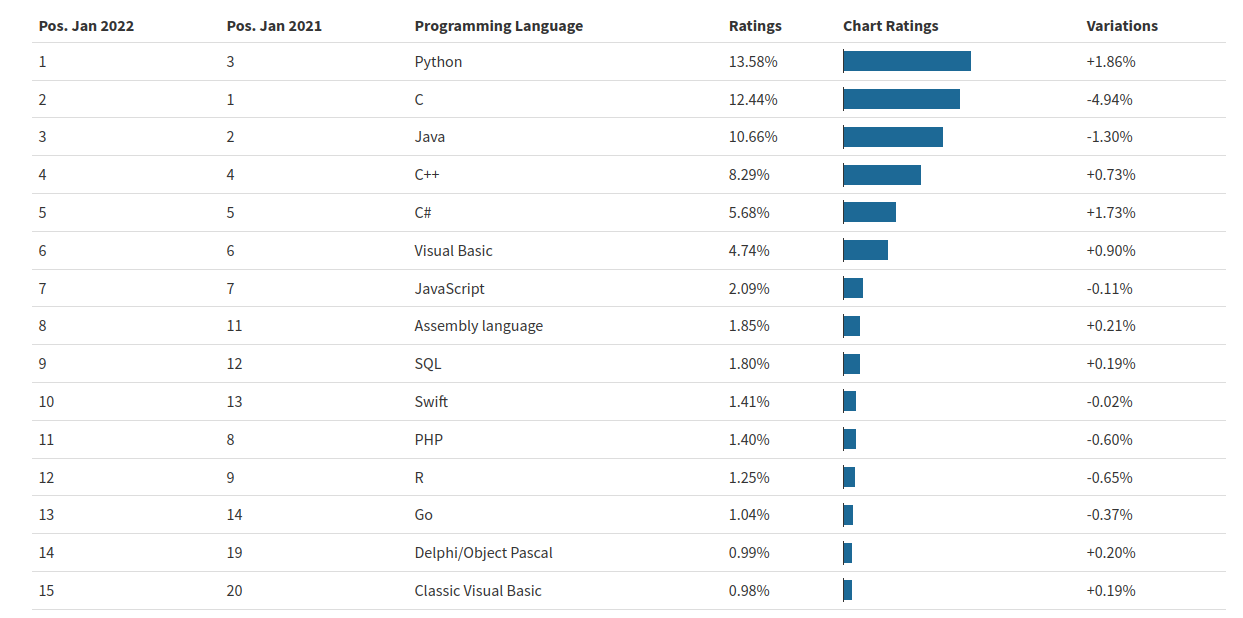
\includegraphics[width=400pt,height=190pt]{slike/most_popular_language.png}
	\label{fig: popular_program_lang}
	\caption{Statistički pregled najpopularnijih programskih jezika (godina 2021--2022). }
\end{figure}

U nastavku navodimo nekoliko važnih informacija vezanih za istoriju razvoja programskog jezika Pajton. 
 
Godine 1989. Guido van Rossum je samoinicijativno započeo rad na kreiranju novog programskog jezika kao poboljšanoj verziji ABC jezika, koji se uglavnom koristio za podučavanje osnovama  programiranja. Van Rossom je izgradio Pajton uzimajući po njemu pozitivne strane ABC jezika kao bazu, a poboljšavajući ili iznova implementirajući lošije koncepte tog jezika. 

 Prva verzija Pajtona, verzija 0.9.0, je objavljena  u februaru 1991. godine.
Pajton 1.0 je objavljen u januaru 1994. godine.  Uključio je nekoliko novih funkcionalnosti, preuzimajući uglavnom dobre koncepte funkcionalnih jezika, kao što su lambda, mapa, filter i funkcije redukcije.
Pajton 2.0 je objavljen 2000. godine i uveo je komprehenziju liste, sakupljač otpadaka i mnoga druga poboljšanja.
Pajton 3.0 je objavljen 2008. godine kao veliko ažuriranje koje je uključilo nekoliko izmjena koje nisu bile kompatibilne sa prethodnim verzijama. \\ 

Glavna odlika verzije Pajton 3.0 bio je pročišćavanje jezika i uklanjanje redudantnih funkcija.
Od pojavljivanja Pajton 3, tim zadužen za razvoj pajtona pušta glavne verzije jezika svakih 18-24 mjeseca. Svaka nova verzija uključuje nove funkcije i poboljšanja, čuvajući kompatibilnosti sa prethodnim verzijama.
Danas se Pajton koristi u gotovo svemu, od razvoja veb aplikacija, do naučnog računarstva, analize podataka, vještačke inteligencije, mašinskog učenja itd. Prednost 
Pajtona je velika i aktivna zajednicu programera koja   svakodnevno doprinose  jeziku kreiranjem biblioteka, frejmvorka i drugih alata. Neke od popularnih biblioteka i frejmvorka za Pajton uključuju NumPy, Pandas, Matplotlib, Django, TensorFlow.


Razvoj Pajtona karakteriše njegova sintaksna jednostavnost, čitljivost i fleksibilnost. Ovi aspekti su pomogli  da Pajton postane popularan jezik među početnicima ali i iskusnijim  programerima.

\section{Osnovne karakteristike}
%Osnovne karakteristika programskog jezika Pajton su: 

\begin{itemize}
	\item Pajton je \textit{jezik visokog nivoa} (eng. \textit{high-level language}):  programski jezik koji je dizajniran tako da ga ljudi lako čitaju, pišu i razumiju. U prevodu,  obezbjeđuje koncepte koje omogućavaju pisanje k\^oda na višem nivou apstrakcije, čime ga približava sintaksi prirodnog jezika, za razliku od jezika niskog nivoa, kao što su asemblerski ili mašinski k\^od.
	\item Pajton je \textit{dinamički tipizirani jezik}. To znači da  se tip varijable određuje u vrijeme izvođenja programa, a ne u vrijeme kompajliranja ili kodiranja. Drugim riječima, tip varijable se može promijeniti tokom izvršavanja programa. Nasuprot ovome, statički tipiziranim jezicima,  tip varijable je fiksiran u vrijeme kompajliranja i nepromjenljiv je tokom vremena izvršavanja. U statički tipiziranim jezicima,  tip svake varijable se mora deklarisati prije upotrebe, a potom kompajler provjerava da li se tip varijable dosljedno upotrebljava u cijelom programu.
	\item Pajton je \textit{objektno-orijentisani jezik}.  Objektno orijentisani programski (OOP) jezik  je tip programskog jezika koji koristi objekte kao svoje osnovne gradivne blokove. Objekti su instance klasa koje enkapsuliraju podatke i operacije (metode) koje se mogu izvršiti na tim podacima. U osnovi,  OOP koncept potiče prirodniji način razmišljanja o problemima tako što ih modeluje u smislu objekata i njihovih interakcija.
	\item Pajton je \textit{skriptni jezik}. Programski jezik koji je dizajniran dijelom za  skriptiranje,   pisanja tipa programa koji se koristi za automatizaciju zadataka, kao što je izvođenje niza naredbi ili manipulaciju podacima. Skriptni jezici se obično interpretiraju, a ne kompajliraju, što znači da se izvorni kod može izvršiti direktno, bez prethodnog prevođenja u mašinski k\^od.  	Jezici za skriptiranje se često koriste za   automatizacija zadataka koji se ponavljaju, pisanje malih potpornih programa ili ugrađivanje funkcionalnosti u drugim aplikacijama. Jedna od glavnih prednosti skriptnih jezika je njihova jednostavnost upotrebe i fleksibilnost.
	\item Pajton posjeduje \textit{aitomatsko čišćenje memorije} (eng. \textit{garbage--collected} language).  Pajton automatski upravlja   identifikovanjem i oslobađanjem memorije koju program više ne koristi.  Oslobađena memorija  stavljanja se na raspolaganje drugim dijelovima programa za korištenje.   Ovaj mehanizam omogućuje  programerima  da se usredotoče na pisanje koda bez vođenja brige o ručnom dodeljivanju i oslobađanju memorije (dok to nije slučaj u, recimo, programskom jeziku $C$).
\end{itemize}

\section{Pregled ugrađenih tipova podataka}

Pajton nudi nekoliko \textit{ugrađenih} (eng. \textit{built-in}) tipova podataka koji su dio osnovnog jezika. Oni su dostupni bez potrebe za dodatnom instalacijom ili bibliotekama. Među ugrađeni tipovima podataka (koji predstavljaju klase), od naročite bitnosti su sljedeći tipovi:

\begin{itemize}
	\item  numerički tipovi: \texttt{int}, \texttt{float}, \texttt{complex};
	 \item  tekstualni sekvencijalni tipovi: \texttt{str}, \texttt{bytes}, \texttt{bytearray};
	\item  sekvencijalni tipovi: \texttt{list}, \texttt{tuple}, \texttt{range}; 
	\item  mapirajući tipovi: \texttt{dict};
	\item skupovni tipovi: \texttt{set}, \texttt{froznenset};
	\item  boolean tip: \texttt{bool};
	\item  binarni tipovi: \texttt{memoryview}.
\end{itemize}


Svaki od ovih tipova posjeduje različite funkcionalnosti za skladištenje i manipulaciju podacima, te se koriste za kreiranje složenih struktura podataka i algoritama. Osim toga, Pajton pruža širok raspon biblioteka koje proširuju funkcionalnost ovih ugrađenih tipova, time omogućavaju kreiranje moćnih i fleksibilnih aplikacija sa lakoćom.

\section{Deklarisanje varijabli i memorijska organizacija}

Dodjela vrijednosti varijablama se izvršava pomoću operatora (dodjele) ``='', kao i kod većine programskih jezika. Da bismo kreirali varijablu, prvo odaberemo naziv varijable, a potom joj dodijelimo vrijednost pomoću operatora ``=''. Npr. za kreiranje varijable pod nazivom \textit{x} sa vrijednošću   5, koristimo sljedeći kod:

\begin{minted}{python}
	x = 5
\end{minted}

Da bismo kreirali varijablu pod nazivom \textit{y} i dodijelili joj stringovnu vrijednost ``abc'', napišemo:
\begin{minted}{python}
	y = "abc"
\end{minted}

Više o cjelobrojnim i stringovnim tipovima podataka biće riječi u nastavku. 
 
Pajton je objektno-orjentisani jezik, gdje se svaka varijabla tretira kao objekat neke klase.  
Objekti koji su varijable sa cjelobrojnom vrijednošću se tretiraju kao objekat tipa \texttt{int}. Dalje, varijabla koja je referencirana na string se tretira kao objekat tipa \texttt{str}.  Inače, gledajući memorijsku organizaciju, pojednostavljeno govoreći, varijable pretstavljaju reference na memorijsko mjesto gdje je upisan sadržaj na koji referenciraju.  
%https://www.analyticsvidhya.com/blog/2021/05/why-you-should-avoid-using-python-lists/
Detaljnije, pajtonov interpreter (o kome će biti više riječi u nastavku) je   napisan u \textit{C}-u, pa su svi pajtonovi objekti prikrivena verzija \textit{C} struktura, stoga  sadrže ne samo svoju vrijednost, već i druge informacije. Objekat nije samo sirovi cijeli broj (ili string ili drugi tip podatka), već pokazivač na složenu \textit{C} strukturu (npr. \texttt{PyLongObject}) koja sadrži nekoliko vrijednosti. Ako istražimo dublje, možemo vidjeti kako ova \textit{C} struktura izgleda.

\begin{minted}{C}
	struct _longobject {
		long ob_refcnt;
		PyTypeObject *ob_type;
		size_t ob_size;
		long ob_digit[1];
	};
\end{minted}
gdje je
\begin{enumerate}
	\item   \textit{\textit{ob\_refcnt}} -- brojač referenci koji upravlja dodjelom i oslobađanjem memorije.
    \item \textit{ob\_type} -- tip varijable.
    \item  \textit{ob\_size} -- veličina podatkovnih članova.
    \item  \textit{ob\_digit} -- čuva stvarnu vrijednost koju varijabla predstavlja.
\end{enumerate}

Sve ove dodatne informacije iziskuju   dodatne troškove u smislu memorijskih i računarskih resursa. Stoga je pajtonov  objekat (nekog tipa podatka)  ništa drugo nego pokazivač na poziciju u memoriji koja sadrži sve informacije o toj varijabli, uključujući količinu memorije sa stvarnom vrijednošću   tog tipa.  Dakle, sve ove dodatne informacije su ono što omogućuje da slobodno kodiramo u pajtonu, bez vođenja brige o tipovima podataka varijabli. Ipak, navedimo da se tip varijable može eksplicitno dodijeliti, kao u narednom primjeru
\begin{minted}{python}
	 x: str = "abc" 
	 y: int = 23
\end{minted}


Jednostavnosti radi, sljedeći k\^od
\begin{minted}{python}
    x = 42
\end{minted}
 pojednostavljeno možemo predstaviti sljedećom vizuelizacijom:
\begin{figure}[H]
	\centering
   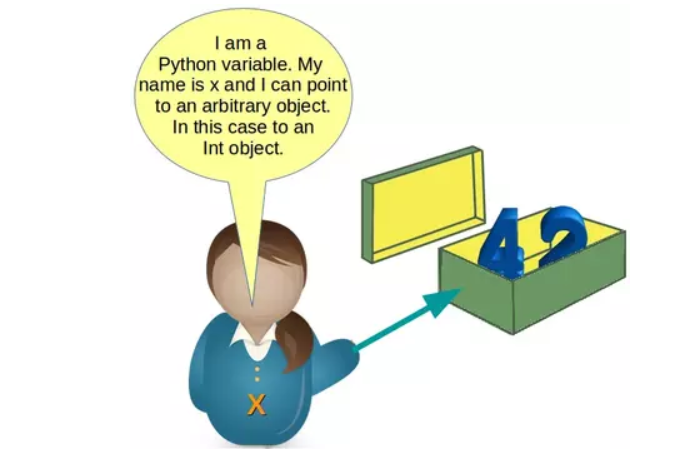
\includegraphics[width=140pt,height=100pt]{slike/variable_object.png}
\end{figure}
U slučaju da dodamo sljedeću liniju   koda 
\begin{minted}{python}
	y = x
\end{minted}
dobijamo situaciju    koja odgovara slici

%point_two_vars.png
\begin{figure}[H]
	\centering
	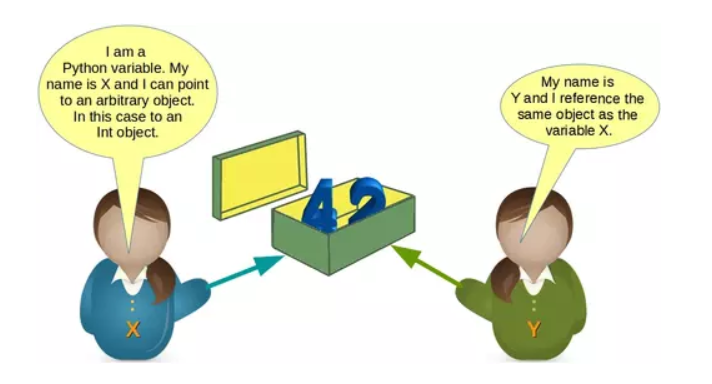
\includegraphics[width=140pt,height=100pt]{slike/point_two_vars.png}
\end{figure}
U slučaju da dodamo sljedeću liniju koda na prethodni k\^od
\begin{minted}{python}
	y = 72
\end{minted}
dobijamo sljedeći prikaz
\begin{figure}[H]
	\centering
	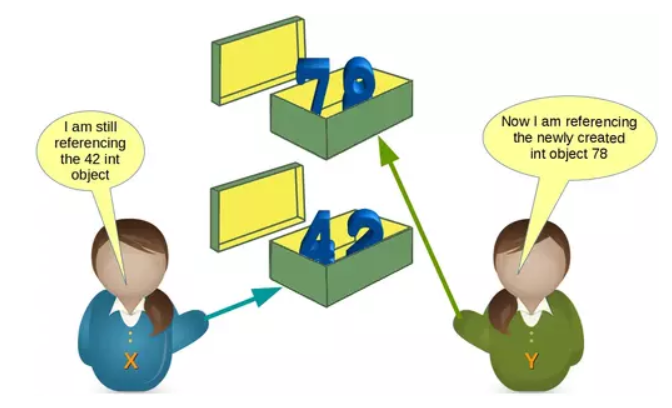
\includegraphics[width=140pt,height=100pt]{slike/vars_different_assigned.png}
\end{figure}
Konačno, ako postavimo y na novu vrijednost, tj.
\begin{minted}{python}
	x = "Text" 
\end{minted}
imamo odgovarajuću sliku 

\begin{figure}[H]
	\centering
	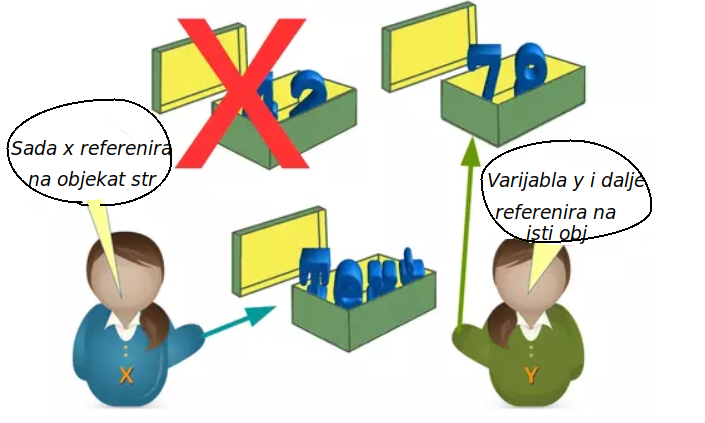
\includegraphics[width=140pt,height=100pt]{slike/varX_different_assigned.png}
\end{figure}

Primijetimo da na memorijsko mjesto gdje je broj 42 bio upisan ne pokazuje niti jedan pokazivač.  Pajton koristi tehniku zvanu \textit{brojač referenci} (atribut \textit{ob\_refcnt}) za upravljanje memorijom. Za svaki objekt, uključujući i složenije strukture kao što su kolekcije, vezuje se jedan broj referenci koji prati broj referenci na objekt. Kada referentni broj postene nula, objekt se briše iz memorije uz pomoć sakupljača otpadaka (eng. \textit{garbage collector}).

Sakupljač otpadaka   povremeno skenira hip u potrazi za objektima sa referentnim brojem nula te ih briše   iz memorije. Na ovaj način se osigurava brisanje i u slučaju  ako postoje kružne reference, gdje dva ili više objekata referenciraju jedan na drugog.

Očitavanje broja memorijske ćelije te heksadekadnog broja na koju pokazuje varijabla $x$ se izvršava pomoću koda:
\begin{minted}{python}
	idnum = id(x) 
	idhex = hex(id(x)) 
\end{minted} 
%https://insideaiml.com/blog/Python-Memory-Management-1176 ==> procitati: BITNO 
 Napomenimo da se ispisivanje rezultata na ekranu vrši pomoću naredbe \emph{print}(). Poruka može biti string ali i bilo koji drugi objekat. Svaki objekat će biti konvertovan u string prije nego što se ispiše na ekran. Ukoliko konverzija nije moguća, javiće se poruka o greški. 
 
 Pisanje komentara u jeziku Pajton je realizovano na više načina: jednolinijski i multilinijski. Jednolinijski komentari počinju sa simbolom tab (\#), nakon čega slijedi opis komentara. U slučaju višelinijskog komentara, početak komentara počinje i završava sa tri uzastopna apostrofa, koji se moraju pravilno uravnati (sa ostatkom k\^oda), da ne bi došlo do pojave sintaksne greške.  
 


\section{Osnovni numerički tipovi podataka}

\textit{Numerički tipovi}. \texttt{int} (skraćeno od \textit{integer}) predstavlja pozitivne ili negativne cijele brojeve, dok \texttt{float} (skraćeno od \textit{floating-point number})  predstavlja realne brojeve sa decimalnim zarezima ili eksponencijalnom notacijom.

Slijede primjeri inicijalizacije ovakvih tipova. 

\begin{minted}{python}
	x = 5        # int 
	y = -3       # int 
	z = 3.14     # float-point number
	w = -0.325   # float-point number
\end{minted}

Nad ovim numeričkim tipovima  je moguće primjenjivati razne aritmetičke operacije, koje su manje-više sintaksno i semantnički iste kao i kod većine ostalih programskih jezika. Napomenimo jednu suštinsku razliku, a to je operator '/' koji podrazumijeva realno dijeljenje, dok '//' označava cjelobrojno dijeljenje. Npr. 5/2 vraća rezultat 2.5, dok 5//2 vraća 2.  

Pored ovih osnovnih aritmetičkih operacija, postoje i druge ugrađene funkcije i metode koje se mogu koristiti sa int i float vrijednostima, kao što su \textit{abs}(), \textit{round}(), \textit{min}(), \textit{max}(), itd.

Numerički tip \texttt{complex} predstavlja kompleksne brojeve koji su dati u obliku a+b\textbf{j}, gdje su $a$ i $b$ oba realni brojevi, dok je  \textbf{\textit{j}} imaginarna jedinica.
\begin{minted}{python}
	x = 1 + 1j 
	y = 2 +  j 
	print(x + y) # Output: 3 + 2j
	z = x + y
	print(z.real) # Output: 3.0
	print(z.imag) # Output: 2.0
\end{minted}
Napomenimo da se kompleksni brojevi mogu inicijalizovati pomoću funkcije  \textit{complex}($x, y$), gdje je $x$ vrijednost realnog, a $y$ vrijednost imaginarnog dijela broja. 


\section{Naredbe grananja i petlje}
%https://petlja.org/biblioteka/r/lekcije/TxtProgInPythonSrLat/02_console-02_console_08_if
U ovoj sekciji navodimo sintaksu naredbe grananja \texttt{if}, te osnovnih petlji \texttt{for} i \texttt{while}. 

Prije toga, u Tabeli~\ref{fig: operatori_poredjenja} navodimo osnovne operatore poređenja u jeziku Pajton. Napomenimo da svaki ovakav izraz vraća bulove konstante \emph{True} ili \emph{False}, u zavisnosti od toga da li je tačan ili ne, respektivno. 

%\begin{figure}[H]
%	\centering
%	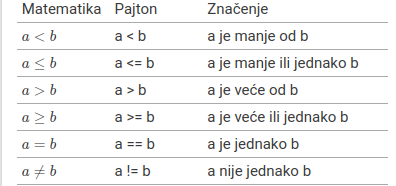
\includegraphics[width=220pt,height=100pt]{slike/operatori_poredjenja.png}
%	\caption{Osnovni operatori poređenja u Pajtonu.}
%	\label{fig: operatori_poredjenja}
%\end{figure}

\begin{table}
		\caption{Osnovni operatori poređenja u Pajtonu.}	\label{fig: operatori_poredjenja}
~	\hline
	\begin{tabular}{lll}
		Matematička notacija & Pajtonova notacija & Značenje \\ \hline
		$a < b$              &  $a < b$           & $a$ je manje od $b$ \\
		 $a \leq b$          &  $a <= b$          &$ a$ je manje ili jednako $b$ \\  
		 $a > b$             &   $a >b$           & $a$ je veće od $b$   \\
		 $a \geq b$          &   $a >= b$         & $a$ je veće ili jednako od $b$   \\
		 $a=b$               &   $a==b$           & $a$ je jednako $b$               \\
		 $a \neq b$          & $a!=b$             &  $a$ nije jednako $b$            \\ \hline    
  	\end{tabular} 
\end{table}

\subsection{Uslovna naredba If}

Sintaksa bazne naredbe \texttt{if} (sa neobaveznom alternativom) je data sa:
\begin{minted}{python}
    if uslov:
        naredba_1
    else:
        naredba_2
\end{minted}

Tok naredbe je sljedeći: ako je \emph{uslov} ispunjen, izvršava se \textit{naredba\_1} (koja može da bude i blok naredbi), inače se izvršava blok \textit{naredba\_2}. Primijetimo pravila uvlačenja ili indentacije (eng. \textit{indentation}) k\^oda pod \texttt{if} blokom koja se moraju poštovati kao sintaksno pravilo. Nakon izvršavanja jedne od naredbi, program izlazi iz ugnježdenog bloka \texttt{if} naredbe, te prelazi na izvršavanje sljedeće naredbe po redu u programu. Kao i u svakom programskom jeziku, tok izvršavanja naredbi je  odozgo prema dolje. Primijetimo da prethodna sintaksa za \texttt{if} radi sam samo dvije alternative. \texttt{If} koji dozvoljava više alternativa se poziva na sljedeći način. 

 \begin{minted}{python}
 	if uslov_1:
 	   naredba_1
 	elif uslov_2:
 	   naredba_2
 	...
 	elif uslov_k:
 	   naredba_k
 	else:
 	    naredba_n
 \end{minted}

Program provjerava redom uslove krenuvši od prvog. U slučaju da se naiđe na  uslov koji je tačan, izvršavaju se odgovarajuće naredbe (u sklopu ugnježdenog  bloka), te program  nastavlja sa izvršavanjem prve naredne naredbe poslije \texttt{if} naredbe pod istim bloku. U slučaju da niti jedan od uslova nije tačan, izvršava se \emph{naredba\_n} (ulazi u ugniježdeni blok pod \textit{else} komandom). Nakon toga, izlazi se iz \texttt{if} bloka te program nastavlja sa prvom narednom naredbom pod istim blokom (uravnanjem).  

\subsection{For i While petlje }

Petlje se koriste za iterativno izvršavanje bloka k\^oda, sve dok se ne ispuni određeni uslov (prekida). Pajton sadrži dvije vrste petlji: \texttt{for} i \texttt{while} petlja.

Petlja se može koristiti \texttt{for} za iterisanje kroz nizovne objekte (kao što je lista, torka, ili string) ili duge iterabilne objekte (rječnici i skupovi).

Sintaksa za petlju \texttt{for} je data sa:
\begin{minted}{python}
     for item in iterable:
         naredba # blok koda koji se izvršava
\end{minted}
gdje je \emph{item} varijabla kojoj se dodjeljuju elementi iterabilnog objekta \textit{iterable} (lista, torka), jedan po jedan, dok se za svaku takvu dodjelu izvrši blok k\^od \emph{naredba}. 
 
Sintaksa za petlju \texttt{while} je data sa:

\begin{minted}{python}
    while uslov:
	  naredba # blok koda koji se izvršava
\end{minted}
\emph{Uslov} podrazumijeva bulov izraz, koji se provjerava prije svakog izvršavanja blok koda \emph{naredba}, koja se potom izvršava ukoliko izraz \emph{uslov} vraća vrijednost  \emph{True}, inače se izlazi iz petlje i tok izvršavanja programa seli na prvu narednu naredbu u programu na istom nivou ugnježdnja kao i \texttt{while} petlja. 

Npr. ispisivanje prvih 10 parnih cijelih brojeva pomoću \textit{while} petlje se dobija izvršavanjem sljedećeg k\^oda.

\begin{minted}{python}
	i = 1
	while i <= 10:
	    print(2*i)
	    i += 1 # Komentar: ekvivalentno dodjeli i = i + 1
\end{minted}

\section{Složene strukture podataka}

Postoji nekoliko osnovih struktura podataka  u Pajtonu koje su fundamentalne za primjenu i rješavanje problema, a to su: stringovi, liste, rječnici (heš mape), torke i skupovi, između ostalih.  %Svaka od ovih struktura  predstavljaja kolekciju elemenata (objekata). 

\subsection{Stringovni tip podataka}

\texttt{Str} je ugrađeni tip podataka (klasa) koji služi za predstavljanje niza Unicode karaktera. Stringovi u Pajtonu su nepromjenjivi; u prevodu, kada se string kreira, ne može se više mijenjati.

\textit{Inicijalizacija}. Da biste se kreirao string, stavimo niz karaktera u jednostruke (') ili dvostruke navodnike (").

\begin{minted}{python}
	string0 = 'hello'
	string1 = "world"
\end{minted}

Višelinijski stringovi se kreiraju koristeći trostruke navodnike. 

\begin{minted}{python}
	multiline_str2 = '''Ovo je
	višelinijski string.'''
\end{minted}

\textit{Metode}.
\begin{itemize}
	\item Konkatenacija stringova se realizuje pomoću operatora '+'. 
	\item Pristupanje karakterima stringa je obezbjeđeno operatorom '[]'. Karakteri stringova su indeksirani brojevima $0, 1,\ldots$ idući od početka stringa ka njegovom kraju, ili sa $-1, -2,\ldots$ idući sa kraja stringa ka početku  (reverzno). 
	\item Rezanje stringa (eng. \textit{slicing}) se realizuje sa `[:]' na sljedeći način:
	\begin{minted}{python}
	 string1 = 'world'
	 substr1 = string1[1:3] # Output: 'or'
	 substr2 = string1[:3] # Output: 'wor'
	\end{minted}
	
	\item  Binarnim operatorom '*' ``lijepimo'' više istih kopija stringa u jedan novi. Drugim argumentom operatora definišemo broj kopija datog stringa.  
	\item Dužina stringa se dobija primjenom funkcije \emph{len}(). 
	\item Brisanje stringa iz memorije se realizuje pomoću ključne riječi \textit{del} koja se pozicionira ispred stringa koji se briše. 
    \item Postoji mnogo pomoćnih funkcija koje nabrajamo ovdje bez detalja: \textit{lower}(), \textit{upper}(), \textit{strip}(), \textit{replace}(), \textit{find}(), itd. 
\end{itemize}

\textit{Memorijska organizacija}. Objekat tipa \texttt{str} je predstavljen nizom Unicode karaktera koji je smješten u neprekidnom bloku memorije. Svaki karakter u tom nizu je predstavljen brojem (kodom) tog karaktera u Unicode standardu. Svaki takav k\^od je predstavljen fiksnim brojem bajtova, u zavisnosti od platforme, što je obično ili 2 ili 4 bajta. Stringovi se često prosljeđuju kao reference na originalni stringovni objekat. %U prevodu,   ako dvije varijable referenciraju na isti string, promjene koje su napravljene putem jedne varijable vidljive su takođe putem druge varijable.

	\begin{figure}
	\centering
	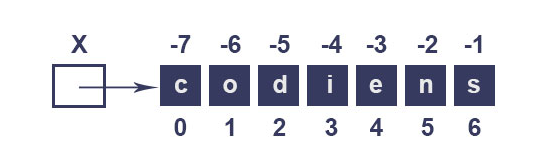
\includegraphics[width=200pt,height=60pt]{slike/str_mem_organization.png}
	\caption{Pojednostavljen prikaz unutrašnje memorijske strukture stringa x=\texttt{code}   u Pajtonu. }
\end{figure}


\textit{Dodatne napomene}. Objekat tipa \texttt{str} u Pajtonu predstavljen je u jeziku \textit{C} kao struktura koja sadrži pokazivač na početak niza podatka (string), kao i druge metapodatke kao što su dužina stringa i trenutna količina dodijeljene memorije za niz.

Definicija odgovarajuće \textit{C} strukture za pajtonov \texttt{str} objekt izgleda ovako:

\begin{minted}{C}
	typedef struct {
		long ob_refcnt;
                PyTypeObject *ob_type;
		Py_hash_t ob_shash;
		Py_UNICODE* st_val
	} PyUnicodeObject;
\end{minted}

Polje ob\_shash se koristi za pohranjivanje keširane vrijednosti niza, a tip Py\_UNICODE se koristi za predstavljanje Unicode znakova u procesu interpretacije programa. %U Pajtonu 3.x, Py\_UNICODE je ekvivalentan ugrađenom tipu \texttt{str} i definisan je kao 2-bajtni ili 4-bajtni neoznačeni cijeli broj.  %u zavinosti od toga kako je Python izgrađen.
 
Jednostavno rečeno, string  pohranjuje  podatke kao neprekidni niz Unicode znakova. %, sa null-terminatorom na kraju. 
Struktura PyUnicodeObject sadrži pokazivač na ove podatke.


Kada se objekt tipa \texttt{str} kreira, prvo se memorija dodjeljuje nizu, a potom se inicijalizuju i metapodaci. Pri nizovnoj manipulaciji, interni bafer se eventualno mijenja kako bi se prilagodio novim podacima. Objekt \texttt{str} je   optimiziran za dijeljenje, kako je već napomenuto. %Preciznije, ako više \texttt{str} objekata sadrži iste znakovne podatke, oni mogu dijeliti isti interni bafer podataka radi uštede memorije. 
 Za stringove je vezan i proces   \textit{interniranja stringova} što označava ponovnu upotrebu postojećih stringovnih objekata umjesto stvaranja novih sa istom vrijednošću. Ovaj proces se izvodi   globalnim keširanjem string objekata i provjerom    keš memorije prije kreiranja novog string objekta. Ako string objekt sa istom vrijednošću već postoji u kešu, on se vraća umjesto kreiranja novog objekta. Ovaj proces štedi memoriju i poboljšava performanse programa, posebno kada se radi sa većim brojem manjih stringovnih objekata.


Potoji nekoliko opcija za ispisivanje rezultata na ekran koristeći ugrađene stringovne funkcije ili specifične tipove stringova. Jedan od načina je pomoću metode \textit{format} ugrađivanjem kao na sljedeći način

\begin{minted}{python}
print("Moje ime je {0} a prezime {1}".format("Marko", "Marković")) 
# metoda ugradjivanja
\end{minted}
Na mjesto $\{0\}$ dolazi prva vrijednost u fukciji \textit{format}, dok na mjesto $\{1\}$ dolazi druga  vrijednost prosljeđena toj funkciji.  

Još jedan metod ispisa se realizuje pomoću formatiranih stringova (tzv. $f$-strings) kao u sljedećem primjeru:
\begin{minted}{python}
	ime = "Marko"
	godine = 32
	print(f"Ime: {ime}, Godine: {godine}")
\end{minted}

\subsection{Liste}
Lista je nehomogena, uređena, indeksirana i promjenljiva kolekcija elemenata. U jeziku Pajton se inicijalizuje kao objekat klase \texttt{list}. Elementi ove kolekcije su indeksirani brojevima, krenuvši od 0. Pajton, za razliku od većine programskih jezika, dopušta indeksiranje negativnim brojevima gdje je u tom slučaju indeks posljednjeg elementa liste -1, pretposljednjeg -2, itd.  

\textit{Inicijalizacija}.

\begin{minted}{python}
	 lista = list()
	 lista1 = ["a", "b", 2.0, 3]
	 lista2 = list(("abc", "sef", 2))
\end{minted}

\textit{Osnovne metode}.   

\begin{itemize}
	\item Operator [$index$]: vraća element liste na poziciji \textit{index} (prvi element liste indeksiran sa 0); 
	\item Operator otkidanja \textit{[indeks1 : indeks2 : k]}: vraća listu uzimajući svaki \textit{k}-ti  element date liste  krenuvši sa elementom na poziciji \textit{indeks1} (0 ako nije naveden),  pa sve do elementa sa indeksom \textit{indeks2} (dužina liste, ako nije naveden) isključno; 
	\item Operator \textit{in}: ispituje da li je element u listi -- vraća \emph{True} ili \emph{False};
	\item \texttt{for} $x$ in \emph{lista}: iterisanje kroz listu prema indeksu; 
	\item \textit{append(elem)}: dodaje se element na kraj liste;
	\item  \textit{remove(elem)}: briše element \textit{elem} iz liste;
	\item  \textit{pop}(): briše posljednji element iz liste;
	\item  \textit{insert(index, elem)}: postavlja element \textit{elem} na poziciji \textit{index} u listi;
	\item  \textit{reverse()}: vraća reverznu  listu date liste; 
	\item \textit{copy}(): pravi kopiju elemenata liste u drugu listu. 
 \end{itemize}

\textit{Memorijska organizacija}.  U pajtonu su liste realizovake kao \textit{dinamički} nizovi. To znači da mogu povećavati ili smanjivati veličinu shodno dodavanjem ili brisanjem elemenata, respektivno. Upravljanje memorijom listi se obezbjeđuje interpreterom.  Pri inicijalizaciji liste, jedan blok memorije se određuje za skladištenje njenih elemenata, pogledati Sliku~	\ref{fig: mem_list_org}.  Veličina ovog bloka memorije zavisi od broja elemenata u listi i korištenog pajtonovog  interpretera.  Npr. u interpreteru (CPython)  memorija je unaprijed dodijeljena u komadima (eng. \textit{chunk}).
%https://rushter.com/blog/python-memory-managment/ https://www.opensourceforu.com/2021/05/memory-management-in-lists-and-tuples/

 \begin{figure}[!ht]
	\centering
	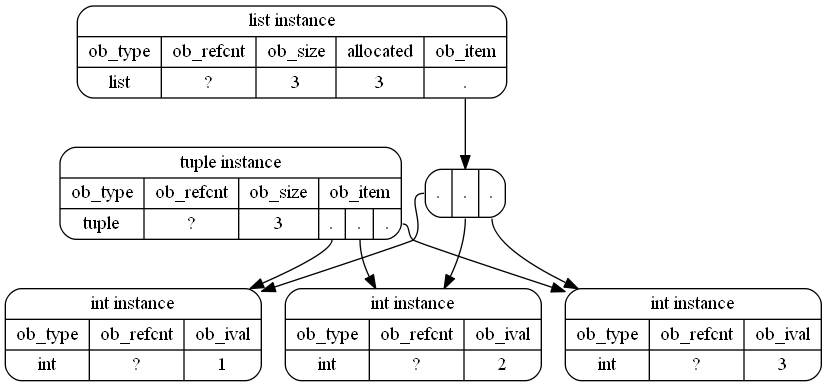
\includegraphics[width=300pt,height=160pt]{slike/img-list-tuple.png}   %list_mem_org.png}

	\caption{Liste u pajtonu: memorijska organizacija i poređenje sa organizacijom torki.} 	\label{fig: mem_list_org}
\end{figure}


%\begin{figure}[!ht]
%	\centering
%	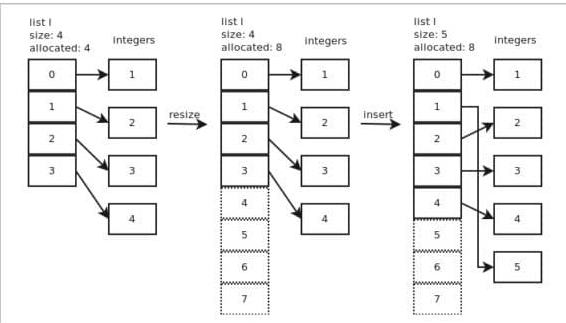
\includegraphics[width=320pt,height=150pt]{slike/list_mem_management.png}
%	\caption{Liste u pajtonu (pojednostavljena prezentacija): dodavanje elementa 5 na početnu listu} 
%\end{figure}%\footnote{Slika sa linka: \url{https://www.laurentluce.com/images/blog/list/list_insert.png}}


 Kada se lista promijeni, interpreter po potrebi dodijeljuje novi blok memorije veće veličine gdje se postojeći elementi liste kopiraju u novododijeljeni blok. Ovaj proces se naziva \textit{realokacija}.  U slučaju kada je potrebno osigurati čuvanje niza, a realokacija nema toliko prostora, stvoriće se nova memorija i kopija što će rezultirati veoma skupom operacijom. Da bismo se to izbjeglo, možemo unaprijed rezervisati potrebnu memoriju. To se može uraditi sljedećim kodom:
 \begin{minted}{python}
    lista =  [None] * max_broj_elemenata
 \end{minted}

Da bi se elementi liste automatski obrisali od strane pajtonovog sakupljača otpadaka, listi je potrebno dodijeliti \texttt{None} vrijednost.  U tom slučaju, svi elementi liste koji nemaju drugih (aktivnih) pokazivača koji pokazuju na date elemente se automatski brišu iz memorije. 

%https://www.analyticsvidhya.com/blog/2021/05/why-you-should-avoid-using-python-lists/
\textit{Dodatne napomene}. Kao što smo napomenuli, za razliku od nizova u programskom jeziku $C$, liste mogu biti heterogene. Međutim, ova fleksibilnost je prilično skupa. Da bi lista bila heterogena, svaki od elemenata liste mora sadržavati informaciju o vlastitom tipu, broju referenci, stvarnu vrijednost na koju pokazuje itd. Drugim riječima, svaka stavka je kompletan pajtonov objekat. Dakle, ako   dalje raščlanimo, lista u pajtonu sadrži pokazivač koji   pokazuje na   blok pokazivača, a unutar svakog bloka,  pokazivači redom pokazuju na odvojeni (puni) pajtonov objekat.  Ako su sve varijable istog tipa, većina ovih informacija postaje suvišna. Alternativa u takvom slučaju je korištenje \textit{array} ugrađenog tipa, o kojem više govorimo u sljedećem odjeljku.   %poput onog koji smo vidjeli ranije. %% Ovo je kao jedna velika lutka!

\subsection{Nizovi: modul Array}

Pajton sadrži ugrađeni modul \textit{array} koji je sličan nizovima u jeziku  \textit{C} ili \textit{C}++. U ovom kontejneru, podaci se smiještaju u neprekidnom bloku memorije. Kao i nizovi u jeziku \textit{C} ili \textit{C}++, oni podržavaju unos jednog tipa podataka u isto vrijeme, dakle nisu heterogeni poput listi u Pajtonu, već homogene strukture. Indeksiranje je slično listama. Tip eleemnata niza mora biti specificiran pomoću koda, koji su pobrojani u Tabeli~ \ref{tab: Tip podataka u objektu array} (podešavajući vrijednost parametra \textit{typecode}). 

\begin{table}[!ht]
	\caption{ Tip podataka u objektu \textit{array}}\label{tab: Tip podataka u objektu array}
	\centering
	\begin{tabular}{llll}  \hline \hline
		\emph{Typecode}      & Tip podatka                  & Pajtonov tip & Veličina (Byte) \\ \hline \hline
		`b' / `B' & signed / unsigned char    & int   & 1 \\
		
		`h' / `H'  & signed / unsigned  short  & int   & 2 \\
        `i' / `I'  & signed / unsigned int     & int   & 2 \\
        `l' / `L'  &  signed / unsigned long   & int   & 4 \\
        `q' / `Q'  & signed / unsigned long long & int & 8 \\
        `f'        & float                       & float & 4 \\
         `F'       & double                      & float & 8 \\ \hline \hline
		
	\end{tabular} 

\end{table}

Da bismo koristili modul \texttt{array}, prvo ga uvedemo sa naredbom \texttt{import}: 
\begin{minted}{python}
 import array 
\end{minted}

\textit{Inicijalizacija. } 
\begin{minted}{python}
    my_array =  array('i', [1, 2, 3, 4, 5])
\end{minted}

\textit{Osnovne metode}. 
\begin{itemize}
	\item Pristup svakom elementu se postiže korištenjem uglaste zagrade; indeksiranje elemenata kreće od 0. 
	\begin{minted}{python}
print(my_array[0])  # Output: 1
print(my_array[2])  # Output: 3
	\end{minted}

\item Modifikacija elemenata se vrži pomoću operatora dodjele (kao i u listama):
\begin{minted}{python}
	my_array[0] = 7
	
	print(my_array)  # Output: array('i', [7, 2, 3, 4, 5])
\end{minted}
\item Funkcije \textit{append}(), \textit{extend}(),  \textit{insert}(), \textit{remove}() i \textit{pop}():  imaju istu ulogu kao i odgovarajuće funkcije u listi. Pogledajmo primjer sa \textit{extend}(): 
\begin{minted}{python}
floats = array('f', [2.0, 3.2, 1.4 ])

tuple_floats = (1.1, 4.1, 5.2, 9.0)

floats.extend(tuple_floats) # dodavanje (kolekcije) elemenata
\end{minted} 
  
\end{itemize}

%\textit{Memorijska organizacija}. 

\subsection{Rječnici}
Rječnici su neuređene, promjenljive, i indeksirane kolekcije elemenata koji su dati u obliku para ključ--vrijednost. Za indeksiranje elemenata upravo služi par ključ--vrijednost koji je jedinstven na nivou objekta ove strukture. Često ime za rječnik je heš mapa. Klasa koja podržava kreiranje objekata koji predstavljaju rječnike je \texttt{dict}. 

\textit{Inicijalizacija}.  

\begin{minted}{python}
	# Vitičaste zagrade
	dct = {"ime": "Mirko", "godine": 30, "grad": "Banja Luka"}
	
	# dict() konstruktor
	dct1 = dict(ime="Mirko", godine=30, grad="Banja Luka")
\end{minted}


\textit{Metode}. 
\begin{itemize}
	\item   Pristup vrijednosti odgovarajućeg ključa:
	
	\begin{minted}{python}
 my_dict = {"ime": "Mirko", "age": 30, "grad": "Banja Luka"}
 print(my_dict["ime"])  # Izlaz: Mirko
	\end{minted}
	
     \item Ažuriranje vrijednosti:
     	
     \begin{minted}{python}
my_dict["godine"] = 31
 
     \end{minted}
U slučaju da dati ključ ne postoji u mapi, par  (``godine'', 31) se dodaje u mapu.  Ako ne želimo posljednji scenario dodavanja, koristi se metoda \textit{update()}.
\item Brisanje elementa: koristi se metod pop(\textit{key}) ili ključna riječ \textit{del}:
 \begin{minted}{python}
	dct = {"ime": "Mirko", "godine": 30, "grad": "Banja Luka"}
	del dct["grad"]
	print(dct)  # Output: {"ime": "Mirko", "godine": 30}
	
	dct = {"ime": "Mirko", "godine": 30, "grad": "Banja Luka"}
	dct.pop("grad")
	print(dct)  #  Output: {"ime": "Mirko", "godine": 30}
 
\end{minted}

\item Provjera da li ključ postoji u heš--mapi: koristimo operator \textit{in}:
 \begin{minted}{python}
     print("ime" in dct)  # Output: True
     print("pol" in dct)  # Output: False
 \end{minted}
\item Ostale korisne metode: 
\begin{itemize}
	\item \textit{len(dct)}: vraća broj elemenata rječnika \textit{dct};
	\item \textit{keys()}: vraća ključeve mape;
	\item \textit{values()}: vraća sve vrijednosti koji dolaze u paru sa ključevima mape
	\item \textit{items()}: vraća sve parove (ključ, vrijednost) date mape:
\end{itemize}
 \begin{minted}{python}
   for x, y in dct.items():
      print("Ključ=", x, " vrijednost=", y)
 \end{minted}
\end{itemize}
\textit{Memorijska organizacija rječnika}.  U Pajtonu, rječnici su implementirani preko heš tabela, koje su predstavljene nizom parova ključ--vrijednost, gdje su ključevi jedinstveni na nivou objekta i koriste se za vraćanje odgovarajućih vrijednosti. Proces unosa, brisanja i traženja elemenata u heš tabeli je obično veoma brz, sa očekivanim konstantnim vremenom za svaku od operacija.
	
	Kada se rječnik kreira u Pajtonu, prvo se heš tabela određene veličine  inicijalizuje u memoriji koja skladišti parove ključ--vrednost. Veličina heš tabele je obično veća od broja inicijalno unesenih elemenata, kako bi se spriječilo često (dinamičko) menjanje veličine heš mape.
	
	Svaki ključ u rječniku se preslikava u cjelobrojnu vrijednost koristeći heš funkciju, a potom se dobijeni broj koristi kao indeks u heš tabeli. Ako se dva ključa heširaju istom heš vrijednosti, dolazi do pojave heš kolizija. Heš tabela tu situaciju rješava tako što oba para ključ---vrijednost čuva u istom indeksu, stvarajući povezanu listu parova ključ--vrijednost, pogledati Sliku~\ref{fig: dict_mem_organization}. Da bi se dohvatila vrijednost pridružena ključu, Pajton prvo izračunava heš vrijednost ključa pa ga potom koristi za lociranje indeksa u heš tabeli u kojoj je pohranjen odgovarajući par ključ-vrijednost. Ako je ključ pronađen, vraća se odgovarajuća vrijednost; u suprotnom se javlja greška.  Kada se novi par ključ-vrijednost treba dodati u rečnik, pajton izračunava heš vrijednost ključa kojeg koristi za pronalazak  indeksa u heš tabeli na čiju poziciju treba da bude pohranjen novi par ključ-vrednost. Ako je indeks već zauzet drugim parom ključ/vrijednost, novi par ključ--vrijednost se dodaje u   listu povezanu sa tim indeksom. Ako broj parova ključ--vrijednost u rječniku premašuje određenu granicu, heš tabela može promijeniti svoju dužinu kako bi se smanjila vjerovatnoća pojavljivanja heš kolizija u svrhu poboljšavanja performansi.
	
	Što se tiče heš funkcija, Pajton koristi heš funkciju zvanu \textbf{hash()} za ugrađene tipove kao što su stringovi (\texttt{str}), cijeli brojevi (\texttt{int}) i torke (\texttt{tuple}). Međutim, za prilagođene objekte, može se definisati vlastita heš funkcija implementacijom metode \_\_\textbf{hash}\_\_(). Funkcija \textbf{hash()}  vraća cjelobrojnu vrijednost koja predstavlja heš vrijednost objekta. Objekti koji se upoređuju kao jednaki treba da imaju istu heš vrijednost, radi ispravnog funkcioniranja rječnika. Napomenimo da za stringove i bajtove, Pajton koristi algoritam \textit{MurmurHash3} za hešovanje vrijednosti. Ovaj algoritam je konstruisan tako da uniformno raspoređuje heš vrijednosti minimizirajući broj kolizija. Za korisnički definisane klase, Pajton koristi zadanu \textbf{hash()} funkciju, koja generiše jedinstvenu heš vrijednost za svaku instancu klase na osnovu memorijske adrese pridružena instanci. Međutim, kao što je ranije rečeno, ovo ponašanje se može nadjačati definisanjem vlastite heš metode. 
	
	
	\begin{figure}
		\centering
		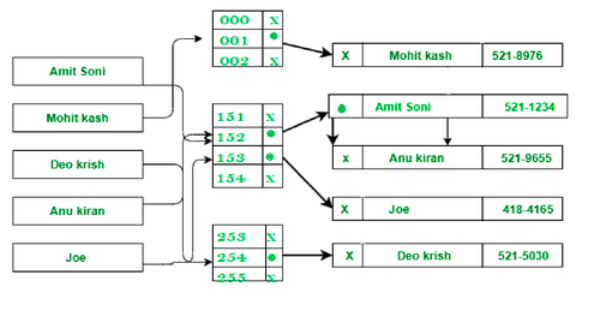
\includegraphics[width=300pt,height=160pt]{slike/dict_mem_organization.png}
		\caption{Pojednostavljen prikaz unutrašnje memorijske strukture jedne heš mape (rječnika) u Pajtonu.\protect\footnotemark}		\label{fig: dict_mem_organization}
	\end{figure}
	%https://www.geeksforgeeks.org/internal-structure-of-python-dictionary/ ==> pročitati
	\footnotetext{Slika posuđena sa https://www.geeksforgeeks.org/internal-structure-of-python-dictionary}
\subsection{Skupovi}

Skupovi  predstavljaju neindeksirane, neuređene, promjenjive strukture podataka čija je osnovna namjena da se na efikasan način izvrši operacija provjere pripadnosti elementa. Ova struktura odgovara matematičkom pojmu skupa, što znači da duplikati u njoj nisu dozvoljeni. Skup može sadržati bilo koju vrstu elementa kao što je \texttt{int}, \texttt{float}, \texttt{tuple}, \texttt{complex}, itd. ali promjenjive kolekcije kao što su iste, rječnici, skupovi ne mogu biti elementi skupa. 


\textit{Inicijalizacija. }
\begin{minted}{python}
	   skup = set()
	   skup1 = {}  #inicializacija praznog skupa
	   skup2 = set((1, 2, "3"))
	   skup3 = set([1, 2, 3])
\end{minted}

\textit{Osnovne metode}. 

\begin{itemize}
	\item \textit{add(elem)}: dodavanje elementa \texttt{elem} u skup; 
	\item \textit{remove(elem)}: brisanje elementa \textit{elem} iz skupa; izbaciće se greška, ukoliko element ne postoji u skupu (\texttt{KeyError} izuzetak, o izuzecima više u narednim sekcijama);
	\item \textit{discard(elem)}: Uklanja element iz skupa ako je prisutan. Ne aktivira grešku ako element nije u skupu;
	\item \textit{pop()}: Vraća i uklanja proizvoljan element iz skupa;
	\item \textit{clear()}: Uklanja sve elemente iz skupa;
	\item \textit{union()}: Vraća novi skup koji je unija elemenata datog skupa i drugog skupa (koji se prenosi kao vrijednost argumenta metoda); kraći zapis ove metode je pomoću znaka  ``$\mid$''.
    \item \textit{intersection()}: Vraća novi skup koji je presjek datog skupa i drugog skupa; kraći zapis ove metode je pomoću znaka ``$\&$''.
    \item \textit{difference()}: Vraća novi skup koji sadrži razliku između datog skupa i drugog skupa. Kraći zapis ove metode je pomoću znaka ``$-$''. 
\end{itemize}
 
 
 


\textit{Memorijska organizacija}. U Pajtonu se skupovna struktura podataka implementira kao neuređena kolekcija jedinstvenih elemenata. Za implementaciju se koristi heš tabela ili rječnik; elementi skupa su ključevi rječnika dok odgovarajuće vrijednosti njima pridružene nisu od važnosti (mogu se pridružiti \textit{None} vrijednosti, koje se za definisanje nula vrijednosti ili vrijednost koja u suštini  označava ``ništa''. Napomenimo da je \emph{None} vlastiti tip podatka (\texttt{NoneType}).).  

Kada se skupu doda novi element, Pajton uz pomoć odgovarajuće heš funkcije izračunava   heš vrijednost koja odgovara  njegovoj  poziciji u heš tabeli. Ako na dobijenoj poziciji nema elementa, novi element se jednostavno dodaje u skup. U slučaju da već postoji element na toj poziciji, provjerava se da li je novi element jednak postojećem (koristeći metodu \_\_eq\_\_()). Ako su dva elementa jednaka, odbija se dodavanje elementa skupu. Inače, po defaultnom principu se element dodaje u linkovanu listu priduržena datom indeksu. Takođe, određeni kompajleri  
koriste algoritam  otvorenog adresiranja da se pronađe pogodna prazna pozicija u heš tabeli gdje bi se potom dodao novi element. 
Otvoreno adresiranje koristi sekvencijalno ispitivanje pozicija da bi se pronašla prazna pozicija u tabeli. Pozicije se provjeravaju sekvencijalno po nekom pravilu dok se ne pronađe prva prazna. Postoji nekoliko pravila  definisanja sekvence probavanja pozicija, kao što je linearno, kvadratno ispitivanje ili dvostruko heširanje. Npr. ako heš pozicija nije prazna, izračunamo sljedeću poziciju u nizu dodavanjem neke konstantne vrijednosti (recimo 1) trenutnoj heš poziciji kretajući se ciklično po pozicijama heš tabele. Ako je trenutna pozicija 4, a konstantna vrijednost 1, sljedeća pozicija koja se ispituje je 5. Ako je sljedeća pozicija prazna,  element se umeće na tu poziciju. Inače, ponovimo prethodni korak dok god se ne pronađe prazna pozicija ili dok se ne pretraži cijela heš tabela. 
 

Slično, u slučaju kada se element uklanja iz skupa, Pajton prvo izračunava njegovu heš vrijednost pri čemu  pronalazi njegovu poziciju u heš tabeli. Ako postoji element na toj poziciji,  provjerava se da li je jednak elementu koji se želi ukloniti. U slučaju da jeste, element se uklanja iz skupa. %Inače,  koristi se otvoreno adresiranje da traži element u ostatku heš tabele.

Pošto su skupovi implementirani kao heš tabele, prosječna vremenska složenost   skupovnih operacija  dodavanja, uklanjanja i provjere pripadnosti je konstanta, dakle $O(1)$. Međutim, u najgorem slučaju, kada postoji mnogo kolizija u heš tabeli, vremenska složenost može da bude i $O(n)$.

Sljedeći kod pokazuje tip strukture podataka u Pajtonu koja predstavlja skup, a to je upravo ugrađeni tip podataka `set'.

\begin{minted}{python}
		s = {1, 2, 3}
		print(type(s)) # <class 'set'>
\end{minted} 


 	\begin{figure}[!ht]
	\centering
	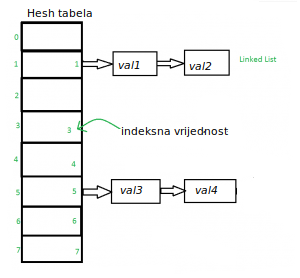
\includegraphics[width=250pt,height=150pt]{slike/set_mem_organization.png}
	\caption{Prikaz unutrašnje memorijske strukture skupa (set) u Pajtonu. }
\end{figure}  %https://www.javatpoint.com/python-set 

\subsection{Torke}
 
 U pajtonu, torka (\texttt{tuple}) je uređena, indeksirana, nepromjenjiva (eng. \textit{immutable}) sekvencijalna kolekcija elemenata, predstavljena jednim objektom u memoriji (na koga pokazuje), dok se ostali objekti određuju implicitnim mehanizmom Pajtona.  Ova struktura dopušta unos duplikata. 
 
 
 \textit{Inicijalizacija}.  
 
 \begin{minted}{python}
 	 my_tuple = ("aa", "bb", 2.0, 3)
 	 my_tuple1 = tuple(["abc", 3.2, 'a'])
 \end{minted}
 
 
 \textit{Osnovne metode}. 
 
 \begin{itemize}
 	\item Pristup elementu torke:
 	\begin{minted}{python}
     my_tuple = (1, 2, 3, 2, 4, 2, 5)
     print(my_tuple[2]) # Output: 3
 	\end{minted}
    \item  Računanje broja pojavljivanja pojedinog elementa:
    
	\begin{minted}{python}    
    my_tuple = (1, 2, 3, 2, 3, 5)
    print(my_tuple.count(2))  # Output: 2
    	\end{minted}
    \item Vraćanje indeksa prvog pojavljivanja elementa u torci:
   	\begin{minted}{python}    
    print(my_tuple.index(2))  # Output: 1
   	\end{minted}
    \item Vraćanje broja elemenata u torci:
       	\begin{minted}{python}    
    	print(len(my_tuple))  # Output: 6
    \end{minted}
    \item Spajanje dvije torke:
  	\begin{minted}{python}    
     my_tuple1 = ("a", "bb", 2)
     my_tuple1 = ("ee", 2, 3.4)
     my_tuple2 = my_tuple + my_tuple1 
     print(my_tuple2) # Output:  ("a", "bb", 2, "ee", 2, 3.4)
    \end{minted}
 \end{itemize}
 
\textit{Memorijska organizacija}.  Pri kreiranju torke, u memoriji se rezerviše fiksna količina memorije za čuvanje svih njenih elemenata. Svaki njen element je pohranjen u kontinualnom  (neprekidnom) bloku memorije,  određen na osnovu tipova podataka sadržani u torci.  Memorijska adresa prvog elementa torke se koristi kao referenca na cijeli objekat. %Pristup pojedinačnom elementu torke zahtijeva izračunavanje memorijske adrese željenog elementa na osnovu njegovog indeksa i veličine   elemenata u torci. Za posljedicu, 
Pristup pojedinačnim elementima torke se izvršava mnogo efikasnije od pristupa elementima liste jer se indeks svakog elementa torke može  izračunati direktno na osnovu njegove pozicije u memoriji. 

Pošto su objekti tipa \texttt{tuple} nepromjenljive strukture, elementi se ne mijenjaju  nakon što su kreirani. Ako je  potrebno izmijeniti određene elemente, treba da se kreira novi objekat torka sa željenim promjenama. Strukture torki su  efikasnije u smislu upotrebe memorije u poređenju sa promjenjivim strukturama podataka (liste, rječnici), jer ne postoji potreba za dodijelom dodatnih memorijskih lokacija da bismo prilagodili promjene u podacima.
 
 %\begin{figure}
 %	\centering
 %	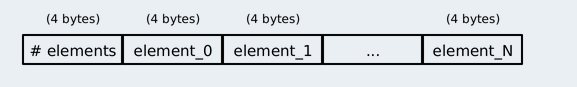
\includegraphics[width=230pt,height=50pt]{slike/tupel_mem_organization.png}
 %	\caption{Pojednostavljen prikaz unutrašnje memorijske strukture jednog objekta torke (tuple) u Pajtonu -- \text{element\_0}, \text{element\_1},$\ldots$ predstavljaju reference na vrijednosti  (reference smještene u neprekidnom bloku memorije). }
 %\end{figure}

\section{Funkcije}

Programski jezik Pajton svaku funkciju predstavlja kao jedan objekat. Prema tome, funkcije se mogu dodijeliti varijablama, proslijediti kao argument  drugim funkcijama, a takođe vratiti kao vrijednost    drugih funkcija.  Preciznije, funkcije su implementirane korištenjem Pajtonove interne klase  \texttt{function}. Ova klasa je dio ugrađenih tipova ovog jezika koja pruža osnovnu funkcionalnost za kreiranje i izvršavanje funkcija. Kada se funkcija definiše, interpreter inicijalizuje novi objekat klase \texttt{function} koji predstavlja tu funkciju -- sadrži informacije o nazivu funkcije, argumentima, k\^odu i drugim metapodacima.

Funkcija je predstavljena blokom k\^oda (nazvan još i definicija tijela funkcije) koji obavlja određeni zadatak a može se pozivati i izvršavati više puta kroz program. Uloga funkcija je da se k\^od učini modularnijim, efikasnijim i čitljivijim, jer omogućavaju  podijelu složenih programa na manje dijelove kojima je lakše upravljati.

Sintaksno, funkcije se definišu pomoću ključne riječi \texttt{def} nakon čega slijedi naziv funkcije, zagrade (u kojima se opciono navode argumenti) pa dvotočka. Tijelo funkcije se uvlači ispod zaglavlja. Naredba \texttt{return} vraća rezultat date funkcije, nakon čega se izlazi iz tijela funkcije. Evo primjera jednostavne funkcije koja računa proizvod dva broja:

\begin{minted}{python}
def proizvod_brojeva(x, y):
    prod = x * y
    return prod
\end{minted}

Da bismo pozvali funkciju, koristimo njen naziv nakon čega u zagradama navodimo vrijednosti svih potrebnih argumenata. Npr. da bismo pozvali funkciju iz prethodnog primjera, pišemo sljedeći k\^od:

\begin{minted}{python}
res = proizvod_brojeva(4, 3)
print(res) # Output: 12
\end{minted}

Funkcije mogu imati defaultne vrijednosti dodijeljene parametarima, koje se koriste ako se funkcija pozove bez specificiranja vrijednosti tim parametrima.  Pogledajmo sljedeći primjer 
\begin{minted}{python}
def umnozi(ime="Mirko", umnozi_puta = 1):
    umnozeno = ime * umnozi_puta
    print(umnozeno)
\end{minted}
Ako se prethodna funkcija pozove bez   vrijednosti argumenata, defaultne vrijednosti se prosljeđuju parametrima (vrijednosti ``Mirko'' i 1, redom), a ispisuje se poruka ``Mirko''. 

Dodatno, funkcije mogu imati i opcione parametre, koji su specificirani pomoću operatora zvjezdice (*) ili dvostruke zvjezdice (**). Sljedeći primjer pokazuje upotrebu ovih operatora:
\begin{minted}{python}
def print_brojevi(*nums):
    for num in nums:
    print(num)
def print_vrijednosti_dict(**key_vals):
    for key, vals in key_vals.items():
         print("Ključevi: ", key, " vrijednosti: ", vals)    

print_vrijednosti_dict({"ime": "Mirko", "prezime": "Mirkovic"})
\end{minted}

Funkcije takođe mogu da vraćaju nekoliko vrijednosti koristeći torke:

\begin{minted}{python}
def visestruko_vracanje(x, y):
    dio = x / y
    ostatak = x % y
    return dio, ostatak

d, o = visestruko_vracanje(10, 3)
print(d, " ", o) # Output: 3 1
\end{minted}

%prenos vrijednosti argumenata:

U jeziku Pajton, vrijednosti argumenata funkcije se prosljeđuju referencom objekta. Dakle, kada se funkcija pozove sa svojim argumentom, referenca na objekt se prosljeđuje funkciji, a ne kopija samog objekta. %Jedino objekti koji su nepomjenljivi (kao što su torke) se proslijeđuju funkciji po vrijednosti (kao ``prava'' kopija a ne originalan objekat). 

Ovo može dovesti do   neočekivanog ponašanja u odnosu na neke druge programske jezike, posebno u radu promjenjivim objektima kao što su liste, rječnici i skupovi. Pogledajmo sljedeći primjer:

\begin{minted}{python}
def dodaj_elem_u_listu(elem, lista):

    lista.append(elem)

lista = list(range(1, 4))
dodaj_elem_u_listu(5, lista)
print(lista)  # Output: [1, 2, 3, 5]
  \end{minted}

Kada se pozove funkcija \texttt{dodaj\_elem\_u\_listu} sa vrijednostima 5 i lista, funkciji prosljeđujemo referencu na objekat lista. Izvršavanjem funkcije, mijenja  se lista dodavanjem novog elementa 5.  U slučaju da ne želimo da funkcija modifikuje (promjenljivi) objekt, treba da se napraviti kopija objekta prije njegovog proslijeđivanja funkciji. Više o kopiranju objekata liste će biti riječi u narednim sekcijama.


Nepromjenjivi objekti kao što su cijeli brojevi, decimalni, stringovi i torke se isto prosljeđuju referencom objekta. Međutim, kako su nepromjenjivi, dakle ne mogu se mijenjati, to znači da sve promjene koje radimo na njima unutar funkcije automatski stvaraju novi objekat (na lokalnom steku).

\begin{minted}{python}
def inkrementiraj(x):
    x += 1
    print("Unutar funkcije:", x)

y = 5
inkrementiraj(y) # Output: 6
print(y) # Output: 5
  \end{minted}
Dakle, varijabla $x$ unutar metoda referiše na novi objekat (i nema veze sa proslijeđenim objektom, osim što su istog naziva). Prema tome, iako se nepromjenljivi objekti takođe prenose  putem reference na objekat, bilo kakvo djelovanje funkcije  neće izmijeniti originalni objekat.  Napomenimo da pomoću ključne riječi \textit{global} ispred naziva varijable možemo preinačiti lokalno ponašanje varijable (koja dozvoljava pristup čitanju sadržaja u funkciji) u globalno (gdje je dozvoljeno i pisanje -- mijenjanje sadržaja na koji varaijabla referencira).  

\begin{minted}{python}
def my_func():
    global x
    x = 10
    print(" Vrijednost unutar funkcije :", x)
x = 20
my_func()
print(x) # Output: 10
\end{minted}

Kao što smo napomenuli, funkcija je jedan objekat te se ona može proslijediti kao vrijednost argumentu druge funkcije, kako je to prikazano sljedećim primjerom
\begin{minted}{python}

def dodaj(a, b):
    return a + b
def primjena(func, x, y):
    return func(x, y)

result = primjena(dodaj, 2, 3)
print(result)  # Output: 5
  \end{minted}

\textit{Anonimne funkcije.}  Anonimne funkcije su definirane pomoću ključne riječi \texttt{lambda}, tako da se ponekad nazivaju i lambda funkcije.  Naziv anonimne funkcije su dobile jer ne zahtjevaju eksplicitnu dodjelu naziva kao u regularnoj funkciji. Sintaksa lambda funkcije je data sa:

\begin{minted}{python}
lambda argumenti: izraz
\end{minted}
Pod \textit{argumenti} se podrazumijevaju argumenti funkcije, a \textit{izraz} predstavlja operaciju koja se izvršava nad ulaznim parametrima. Funkcija vraća rezultat koji se dobija izvršavanjem tog izraza uvrštavajući vrijednosti proslijeđenih argumenata. 

Sljedeći primjer daje lambda funkciju za operaciju sabiranja.
\begin{minted}{python}
suma = lambda x, y: x + y
print(suma(4, 3)) # Output: 7
\end{minted}

Ovdje je lambda funkcija pridružena varijabli \textit{suma}, što je moguće jer je svaka funkcija u programskom jeziku Pajton objekat. Potom su ovoj funkciji proslijeđene reference (na vrijednosti 4 i 3). 

Lambda funkcije su često korisne u situaciji kada je potrebno definisati jednostavne (i sadržinski male) funkcije ukoje se koriste u kraćem periodu pa nema smisla da se definišu kao funkcije punog imena. Pored toga, lambda funkcije su često korištene u kombinaciji sa funkcijama, koje su opštepoznate iz funkcijskih jezika, kao što su: \textit{map}(), \textit{filter}(), \textit{reduce}(), o kojima će biti više riječi u nastavku ove knjige, konkretno u Sekciji~\ref{sec:concepts-pyhton}. 


\section{Kompajliranje i izvršavanje programa}

\subsection{Stek vs. Hip} 


Prilikom izvođenja programa, računarska memorija se dijeli na različite dijelove. Dva važna memorijska dijela su \textit{stek} i \textit{hip} memorija. 

%K\^od sekcija pohranjuje instrukcije koda u obliku koji mašina razumije. Mašina slijedi upute u sekciji koda. Shodno instrukcijama, 
Pajtonov interpreter učitava funkcije i lokalne varijable (reference) u memoriju steka. 
Stek memorija je statična i privremena. Statična znači da se veličina objekata pohranjenih u steku ne može da bude promijenjena. Riječ privremeno znači da čim pozvana funkcija vrati svoju vrijednost, funkcija i   varijable vezane za funkciju se uklanjaju sa steka. Pristup memoriji steka nije direktno obezbjeđen programeru, već  briga o ovom dijelu memorije je dodijeljena Pajtonovom interpreteru i OS-u.  Količina memorije koja  se dodijeljuje je poznata interpreteru i kad god se pozove funkcija, njene varijable zauzimaju memoriju koja se rezerviše na steku.
% Pratimo: https://towardsdatascience.com/python-memory-and-objects-e7bec4a2845ž
% O steku i hipu: https://www.geeksforgeeks.org/how-are-variables-stored-in-python-stack-or-heap/

\begin{minted}{python}
	def func():
	
	    # Ove varijable dobijaju memoriju 
	    # alociranu na steku 
	    a = 10
	    b = []
            c = "abc"
\end{minted}

Kao što smo prethodno rekli, varijable (ili reference generalno) skladište samo memorijske adrese objekata. Dakle, postavlja se pitanje gdje se skladište sami objekti? Oni se nalaze u drugoj memoriji koja se zove \textit{hip} (eng. \textit{Heap memory}). Napomenimo da riječ hip nema veze sa istoimenom strukturom podataka  već  zbog dostupnosti gomile memorijskog prostora u svrhu pohranjivanja i brisanja objekata.   Za pohranjivanje objekata potrebna nam je memorija sa dinamičkom alokacijom  -- veličina memorije i objekata se mogu mijenjati. Pajtonov interpreter je zadužen za aktivno dodjeljivanje memorije hipu (Primijetimo da u jeziku $C/C$++ to  se izvršava od strane programera!). Varijable koje su pohranjene u memoriji hipa su: ($i$)   izvan poziva metoda ili funkcija ili ($ii$) dijele se unutar više funkcija, dakle globalnog svojstva.

\begin{minted}{python}
     # Memorija za 10 brojeva
     # je alocirana na hipu
     a = [0]*10     
\end{minted}


Napomenimo još jednom da Pajton koristi algoritam za sakupljanje otpadaka (eng. \textit{garbage collector}) koji održava memoriju hipa čistom, periodično uklanjajući  objekte koji se više ne koriste.



\subsection{Kompajliranje i izvršavanje}

Proces kompilacije   i izvršavanja k\^oda u programskom jeziku Pajton je kompleskan proces kojeg nećemo izlagati u svim detljima nego ćemo ukratko navesti osnovne principe na kojima je baziran ovaj proces. On uključuje četiri osnovna koraka.
\begin{itemize}
	\item \textit{Leksička analiza} -- Izvorni k\^od se prvo prosljeđuje leksičkom analizatoru,  koji razlaže k\^od na pojedinačne tokene kao što su ključne riječi, identifikatori, operatori, itd.
	\item \textit{Parisiranje} -- Tokeni se zatim prosleđuju parseru, koji koristi gramatiku bez konteksta za izgradnju \emph{apstraktnog sintaksnog stabla} (AST) koje predstavlja strukturu k\^oda. U detalje ovog procesa nećemo ulaziti jer izlazi iz domena ove knjige.
	\item \textit{Kompilacija} -- AST se kompajlira u bajtkod, koji je jezik nižeg nivoa,   nezavisan od platforme.  Ovaj bajtkod se čuva u .\textit{pyc} fajlovima kojeg izvršava   Pajtonova \textit{virtuelna mašina} (VM).
	\item \textit{Izvođenje} -- Pajtonova VM izvršava dobijeni bajtkod tako što ga interpretira generišući \textit{mašinske instrukcije} u hodu. Bajtkod se izvršava u zaštićenom okruženju virtuelne mašine (obezbjeđuje sigurnost i izolaciju od osnovnog OS-a).  
	
\end{itemize}
Napomenimo da tokom procesa izvršavanja, interpreter izvodi nekoliko optimizacija u k\^odu (npr. eliminaciju repne rekurzije), što može poboljšati performanse k\^oda.
%https://www.geeksforgeeks.org/what-makes-python-a-slow-language/
\begin{figure}[H]	
	\centering
	
	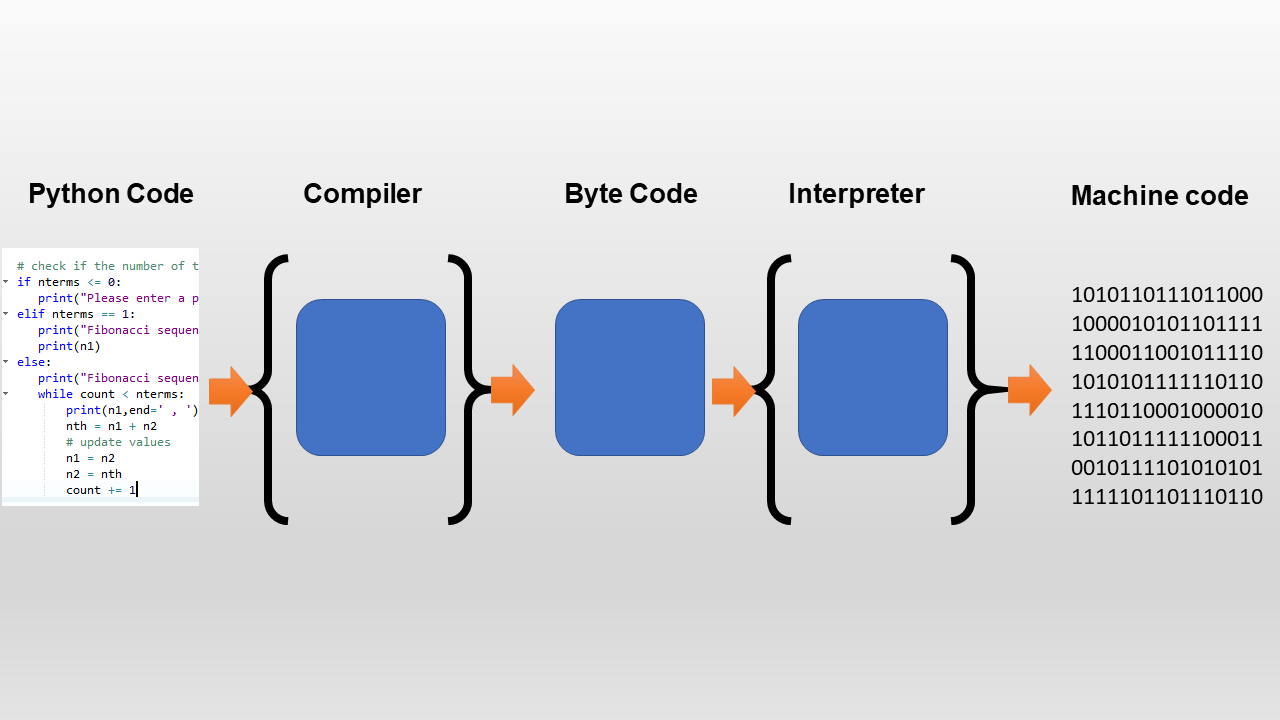
\includegraphics[width=350pt,height=170pt]{slike/python-code-copiler-machine-code.png}%compile_python.png}
\caption{Vizuelizacija procesa izvršavanja k\^oda u Pajtonu.\protect\footnotemark}
\label{fig:comp_interpreting}
\end{figure}

\footnotetext{Slika sa linka: {https://www.astateofdata.com/python-programming/can-python-be-compiled/}}
%%https://www.astateofdata.com/python-programming/can-python-be-compiled/
% Na osnovu prethodnog, pajton je i kompajliran i interpretiran jezik. 
%https://www.astateofdata.com/python-programming/can-python-be-compiled/ ==> procitati ovdje...

Recimo sada malo više o Pajtonovoj virtuelnoj mašini (PVM), bazičnoj komponenti ovog programskog jezika. Kako smo naveli, PVM je odgovorna za interpretiranje bajtkoda i izvršavanje k\^oda. Bajtkod se generiše od strane pajtonovog kompajlera (npr. CPython, Brython) pri kompajliranju izvornog k\^oda.

Ključne uloge PVM su navedene u nastavku. 
\begin{itemize}
\item \textit{Kompatibilnost između platformi}: PVM omogućava izvršavanje pajtonovog k\^oda na više različitih platformi bez ponovne kompilacije. Ovo olakšava pisanje i distribuciju aplikacija.
\item \textit{Poboljšane performanse izvršavanja}: PVM koristi bajtkod  interpreter, koji je brži od direktnog interpretera izvornog k\^oda. PVM može koristiti \textit{Just-In-Time} (JIT) kompilaciju za dalje poboljšanje performansi.
\item \textit{Dinamičko tipiziranje}: Pajton je dinamički tipiziran jezik, što znači da se tip varijable dodjeljuje u vremenu izvođenja programa. PVM je dizajnirana da efikasno upravlja ovim procesom.
\item  \textit{Upravljanje memorijom}: PVM automatski upravlja memorijom, što može olakšati pisanje sigurnog memorijskog k\^oda. PVM  automatski oslobađa memoriju koja se više ne koristi.
\item \textit{Lak pristup eksternim bibliotekama}: PVM se intenzivno koristi u pajton ekosistemu, koji uključuje veliki broj otvorenih biblioteka. Ove biblioteke pružaju širok spektar funkcionalnosti vezano za  veb programiranje, mašinsko učenje, itd. Importovanje biblioteka se vrši pomoću naredbe \texttt{import}. 
\end{itemize}


Na osnovu izloženog, Pajton je i kompajlabilan (prevodi se u bajtni k\^od) i interpretiran jezik. 
Vizuelizaciju procesa prevođenja programa možete da vidite na Slici~\ref{fig:comp_interpreting}.


\section{O nekim programskim konceptima i ugrađenim funkcijama} \label{sec:concepts-pyhton}

U ovoj sekciji ćemo demonstrirati rad sa nekoliko bitnih i često korištenih ugrađenih funkcija koje su dio standardne pajtonove biblioteke. Dodatno, biće objašnjen i koncept komprehenzije liste (eng. \textit{list comprehension}) koji  doprinosi većoj modularnosti k\^oda i približava ga konceptima funkcijskih programskih jezika (kao što je Haskel). 

\subsection{Komprehenzija liste}

Komplehenzija liste predstavlja koncizan način za kreiranje liste. To je konstrukcija koja omogućava kreiranje liste u jednoj liniji k\^oda, umjesto da se koriste petlje (i odgovarajuće metode) za iterativnu konstrukciju liste.

Osnovna sintaksa ovog koncepta je sljedeća:

\begin{minted}{python}
	lista = [expr  for item in iterable]
\end{minted}
Ovdje \textit{expr} označava izraz koji se izračunava do vrijednosti koja se smiješta u listu.
Dalje, \textit{item} je varijabla koja  uzima vrijednosti iz (iterabilnog) objekta \textit{iterable}.  Rezultat primjene je nova lista sastavljena od  vrijednosti dobivenih primjenom izraza  \textit{expr} na svaki elemenat objekta \textit{iterable}.

Npr.\ recimo da želimo kreirati listu prvih 10 parnih brojeva. K\^od bi mogao da ide ovako:

\begin{minted}{python}
	parni = []
	for i in range(1, 11):
	    parni.append(2*i)
\end{minted}

Kraći zapis koda, pomoću komprehenzije liste, izgleda ovako:


\begin{minted}{python}
	parni = [2*i for i in range(1, 11)]
\end{minted}
Takođe se  uslovni izrazi  mogu uključiti u koncept komprehenzije liste. Sintaksa je sljedeća:

\begin{minted}{python}
	lista = [expr  for item in iterable if uslov]
\end{minted}
U ovom slučaju, uslovna komanda se odnosi na elemente koje uzima varijabla \textit{item} -- to su samo oni koji zadovoljavaju \textit{uslov}. 

\subsection{Funkcije map, filter, reduce}

Funckije \textit{map}(), \textit{filter}() i \textit{reduce}() su ugrađene funkcije koje se opšteprisutne u funkcijskom programiranju. One su korisne kao alati za obradu podataka, posebno kada se radi o velikim skupovima podataka.

Funkcija \textit{map}() uzima dva argumenta: funkciju i iterabilni objekat. Primjenjuje funkciju  na svaki element iterabilnog objekta i vraća iterator na naredni element kao rezultat. 

\begin{minted}{python}
     brojevi = [1, 2, 3, 4, 5]
     doubled = map(lambda x: x*2, brojevi)
     print(list(doubled))  # Output: [2, 4, 6, 8, 10]
\end{minted}


Funkcija \textit{filter}() uzima dva argumenta: funkciju koja vraća logičku vrijednost i iterabilni objekat. Primjenjuje funkciju na svaki element iterabilnog objekta i vraća iterator na one elemenate za koje je funkcija vratila \emph{True}. 
\begin{minted}{python}
	brojevi = [1, 2, 3, 4, 5]
	parni = filter(lambda x: x % 2 == 0, brojevi)
\end{minted}

Funkcija  \textit{reduce}(): Sintaksa ove funkcije je

\begin{minted}{python}
	reduce(func, iterable[, initial ])
\end{minted}

Ona uzima dva (obavezna) argumenta,  funkciju i iterabilni objekat, te opciono \textit{initial}. Inicijalno, funkcija \textit{func} se primjenjuje na element \emph{initial} i prvi elemenat iterabilnog objekta, te vraća rezultat. Potom,    primjenjuje istu funkciju na vraćeni rezultat i sljedeći element, i tako dalje, sve dok se svi elementi \emph{iterable} objekta ne obrade. 

Pogledajmo sljedeći primjer: 
\begin{minted}{python}
from functools import reduce #uključianje konkretne metode iz modula 

numbers = [1, 2, 3, 4, 5]
product = reduce(lambda x, y: x * y, numbers, 1)
\end{minted}

Ovo će primijeniti funkciju množenja na prva dva elementa liste, zatim na rezultat i sljedeći element, i tako dalje, sve dok se svi elementi ne obrade, što rezultira proizvodom svih brojeva liste. Pirmijetimo da funkcija \textit{reduce}() nije dio standardnog Pajtonovog modula, već se mora uključiti direktno pozivom \texttt{functools} modula. Više o modulima i radu sa njima ćemo govoriti u narednim sekcijama.



\subsection{Funkcije zip, enumerate i sort}
Funkcije  \textit{zip}() i \textit{enumerate}() su ugrađene funkcije korisne za obradu i iterisanje preko lista ili drugih iterabilnih objekata.

Funckija \textit{zip}() uzima jedan ili više iterable objekata i vraća iterator koji generiše torke koje sadrže uparene elemente svakog iterabilnog objekta (prvi elementi svih listi u jednu torku, drugi elementi svih listi u novu torku, itd.). Sintaksa funkcije je:
\begin{minted}{python}
zip(iterable1, iterable2, ...)
\end{minted}
gdje su \emph{iterable1}, \emph{iterable2},... iterablini objekti. 

Npr. ako imamo dvije liste brojeva i želite da uparite odgovarajuće elemente, imamo sljedeći kod:
\begin{minted}{python}
list1 = [1, 2, 3, 4]
list2 = [5, 6, 7, 8]
parovi = zip(list1, list2) 
print(list(parovi)) # Output: (1, 5), (2, 6), (3, 7),  (4, 8).
\end{minted}
Funkcija \textit{enumerate}() uzima iterativni objekat i vraća iterator koji generiše parove koji sadrže indeks elementa i sami element. Sintaksa funkcije je:
\begin{minted}{python}
	enumerate(iterable, start=0)
\end{minted}
gdje je \textit{iterable} jedan iterabilni objekat, a \textit{start} je početna vrijednost indeksa (podrazumijeva se 0). Pogledajmo sljedeći primjer. 

\begin{minted}{python}
voce = ['jabuka', 'banana', 'kruska', 'breskva']
for i, vocka in enumerate(voce):
    print(i, vocka) # (0, 'jabuka'), (1, 'banana'),
    # (2, 'kruska'), (3, 'breskva')
\end{minted}

Funkcija \textit{sort}() je ugrađena funkcija koja se koristi za sortiranje elemenata   liste po nekom kriterijumu. Ona je metoda liste koja ne vraća ništa već je njen zadatak sortirati listu (u memoriji koja joj je već dodijeljena).

Sintaksa ove funkcije data je u nastavku 
\begin{minted}{python}
	sort(reverse=False, key=None)
\end{minted}

Argument \textit{reverse} prosljećuje poredak sortiranja u listi na način da ukoliko mu je dodijeljena vrijednost \emph{True}, lista će biti sortirana u opadajućem, a inače (po defaultu) redoslijed sortiranja je rastući. Kriterijum sortiranja (kao funkcija) se proslijeđuje argumentu funkcije \textit{key}. Primijetimo da ukoliko se kriterijum sortiranja ne proslijedi eksplicitno, Pajton koristi interne relacije poretka za tip objekata, ukoliko su oni uporedivi (predefinisanom relacijom totalnog uređenja, kao kod osnovnih tipova podataka). U slučaju da objekti nisu uporedivi, vraća se poruka o greški.  Jedna od mogućih grešaka koja se može javiti je sljedeća:
\begin{minted}{python}
TypeError: '<' not supported between instances of 'str' and 'int'
\end{minted}


Primjer sortiranja numeričkih vrijednosti je dat k\^odom:
\begin{minted}{python}
brojevi = [6, 3, 8, 3, 1, 7]
brojevi.sort(reverse=True)
print(brojevi) # Output: [8, 7, 6, 3, 3, 1]
\end{minted}
  Takođe je moguće koristiti funkciju \textit{sorted}() za sortiranje liste i vraćanje nove sortirane liste bez mijenjanja originalne liste:
\begin{minted}{python}
brojevi = [5, 2, 8, 3, 1, 7]
sort_brojevi = sorted(brojevi)
print(sort_brojevi)
\end{minted}

Postoji i niz drugih pomoćnih opštekorišćenih funkcija, koje ćemo pobrojati u nastavku bez ulaska u detalje o njihovoj sintaksi i korišćenju:
\begin{itemize}
	\item \textit{sum}(iterable): vraća sumu vrijednosti elemenata iterabilnog objekta \emph{iterable};
	\item \textit{eval}(expr): vraća vrijednost izraza \emph{expr} zapisan u stringovnom zapisu;
	\item \textit{round}(num, dec\_place): zaokruživanje decimalnog broja na proslijeđen broj decimala;
	\item \textit{max}(iter): vraća broj maksimalne vrijednosti među proslijeđenim brojevima;
	\item \textit{abs}(num): vraća apsolutni vrijednost broja. 
\end{itemize}
\section{Uopšteno o modulima}

\textit{Modul} je datoteka koja sadrži Pajtonove definicije i naredbe. Naziv datoteke je naziv modula sa sufiksom .\textit{py}.

Modul može sadržati različite definicije kao što su funkcije, klase i varijable, koje se mogu uvesti i koristiti u drugim Python skriptama ili modulima. To olakšava organiziranje i ponovnu upotrebu k\^oda (eng. \emph{re-usability}) u različitim projektima.

Da bismo koristili modul u Pajtonu, prvo ga trebamo uvesti pomoću naredbe \texttt{import}. Npr. ako postoji modul pod nazivom \textit{mojmodul}.py, uvodimo  ga na sljedeći način:
\begin{minted}{python}
	import mojmodul
\end{minted}


Nakon što je modul uveden, pristupamo njegovim funkcijama, klasama i varijablama pomoću notacije tačka. Npr. ako \textit{mojmodul} sadrži funkciju pod nazivom \texttt{mojafunkcija}, poziva se ovako:
\begin{minted}{python}
mojmodul.mojafunkcija()
\end{minted}

Takođe se može koristiti i ključna riječ \texttt{from} za uvoz određenih funkcija ili klasa iz modula:
\begin{minted}{python}
from mojmodul import mojafunkcija
\end{minted}

Ovo će omogućiti direktno korištenje funkcije bez potrebe za tačaka notacijom:

\begin{minted}{python}
mojafunkcija()

\end{minted}

Pajton dolazi s velikim brojem ugrađenih modula, među kojima izdvajamo \texttt{math}, \texttt{random}, \texttt{datetime}, \texttt{os} i \texttt{numpy} o kojima će biti riječi u nastavku ove sekcije. Ovi moduli se uključuju direktno sa instalacijom jezika Pajton.
 
%Napomenimo da se mogu kreirati i vlastite module koji prvenstveno služe da bolje organizovanje i reiskorištavanje vlastitog koda.

\subsection{Instaliranje eksternih modula} 


Da bismo instalirali eksterne module u Pajtonu,   koristi se menadžer paketa \textit{pip}, koji dolazi direktno sa instalacijom Pajtona. 

Koraci za instaliranje eksternih modula pomoću \emph{pip}-a su dati u nastavku. Otvorimo terminalnu konzolu i upišimo naredbu \textit{pip install naziv\_modula}, gdje je \textit{naziv\_modula} (obično) odgovara nazivu  modula kojeg želimo instalirati. Npr. da bismo instalirali modul \textit{requests}, pišemo:
\begin{minted}{python}
    pip install requests
\end{minted}

Pritiskom tastera Enter, instalacija se pokreće; pip automatski preuzima modul sa PyPI (eng. \textit{Python Package Index}) i instalirati ga u trenutno pajton okruženje. PyPI je repozitorij softverskih paketa koji su napisani u Pajtonu, a besplatno su dostupni za korištenje. Sadrži više od 300,000 paketa koje možemo instalirati pomoću \textit{pip} menadžera.


Kada proces instalacije modula uspješno završi, modul se može uključiti u naš program pomoću naredbe \textit{import}. Npr. da bismo koristili modul \textit{requests}, pišemo sljedeće:
\begin{minted}{python}
    import requests
\end{minted}
Takođe se možete navesti određena verziju modula za instalaciju dodavanjem  ``==''  iza kojeg slijedi broj verzije modula kojeg želimo da instaliramo. Npr. da bismo instalirali verziju 2.2.1 modula \textit{requests},  pisali bismo:
\begin{minted}{python}
pip install requests==2.2.1
\end{minted}


\subsection{Modul Math}

\texttt{Math} je modul koji služi za rad sa različitim matematičkim funkcijama i konstantama. Da bismo koristili matematički modul u svom programu, prvo morate uvesti pomoću naredbe \textit{import math}.

Nakon što se uveze ovaj modul, omogućeno je korištenje njegovih funkcija i konstanti u k\^odu. Navedimo nekoliko konkretnih primjera. 

\begin{minted}{python}
import math

# Računajmo korjen broja
x = math.sqrt(25)
print(x)  # Output: 5.0

# Konstanta Pi
pi = math.pi
print(pi)  # Output: 3.141592653589793

# Računanje sin 
sin_angle = math.sin(45)
print(sin_angle)  # Output: 0.7071067811865475
\end{minted}

Neke od češće korištenih metoda ovog modula su:   \textit{sqrt}(), \textit{pow}(), \textit{log}(), \textit{exp}(), \textit{log10}(), \textit{floor}(), \textit{ceil}(), \textit{fabs}(), \textit{gcd}(), \textit{dist}() – Euklidova udaljenost između dvije tacake (predstavljene kao torke, ili liste), \textit{isnan}(), \textit{sin}(), \textit{cos}(), \textit{tan}(), \textit{sinh}(), \textit{asin}(), među ostalim metodama.

U nastavku navodimo jednu od internih implementacija korjene funkcije \textit{sqrt}() broja $x\geq 0$. Ona je implementirana  korištenjem algoritma koji se zove \textit{Babilonova metoda}, poznata i pod nazivom Heronova metoda. Algoritam je numerička iterativna metoda koja aproksimira kvadratni korijen broja \textit{x} uzimajući prosjek prethodne aproksimacije i vrijednosti količnika broja $x$ i vrijednosti dobijene u prethodnoj aproksimaciji. Proces se nastavlja sve dok aproksimacija nije dovoljno precizna. Preciznije, primjeljuje se naredna rekurzija:
\begin{center}
	$y_{n+1}= \frac{1}{2}(y_n + \frac{x}{y_n})$
\end{center}
za neki proizvoljan inicijalni korak $y_0> 0$. Trivijalno, za $x=0$, vraća se vrijednost 0. Algoritam se izvršava dok se ne postigne unaprijed zadana preciznost $\epsilon$ broja $x$, tj. dok ne bude ispunjeno $|y_{n+1} - \frac{x}{y_n}| \leq \epsilon$. 
\subsection{Modul Random}

Modul \texttt{random}  pruža skup funkcija za generiranje (pseudo-)slučajnih brojeva,   korisni u različitim aplikacijama kao što su  kriptografija i razvoj igara.

Navedimo neke osnovne funkcije ovog modula.

\begin{itemize}
	\item   \textit{random}():  slučajan nasumični \textit{float} broj između 0 i 1, uključujući 0, ali isključujući 1;
	\item \textit{randint}(\emph{a, b}):  generiše nasumični cijeli broj između $a$ i $b$, uključujući oba broja,  $a$ i $b$.
	\item  \textit{choice}(\emph{seq}):  vraća slučajan element datog niza \textit{seq}; 
	\item \textit{shuffle}(\emph{seq}): nasumično permutuje elemente u datom nizu \textit{seq};
	\item \textit{sample}(\emph{populacija, k}): Ova funkcija vraća nasumično odabran uzorak od $k$ elemenata iz date populacije  \textit{populacija} bez zamjene;
	\item \textit{seed}($a$=None): inicijalizuje generator slučajnih brojeva. Ako argument \textit{a} nije naveden, koristi se sistemsko vrijeme.
 
\end{itemize}

Implementacija funkcije \textit{random}() u Pajtonu koristi algoritam generatora pseudo-slučajnih brojeva, koji je deterministički a generiše niz brojeva koji se čini slučajnim. Algoritam koji se koristi u funkciji \textit{random}() je algoritam \textit{Mersenne Twister},  široko korišten   za generiranje pseudo-slučajnih brojeva.

Algoritam \textit{Mersenne Twister} generiše niz 32-bitnih cijelih brojeva koristeći specijalni linearni pomaknuti (eng. \textit{shift})  registar povratne sprege,  koji koristi operacije isključivanja ili (XOR) za generiranje izlaza. Algoritam koristi veliki prost broj koji se zove \textit{Mersenov} prost ($2^{19937}-1$) kao modul, koji osigurava da generisani niz ima dug period   i dobra statistička svojstva. Inače, algoritam su razvili Makoto Matsumoto i Takuji Nishimura 1997. godine. Drugi generator  koji se može koristi je prosti \textit{linerarni kongruentni generator} 
koji generiše  slučajne brojeve po rekurziji
$$ x_{n+1} = (a x_n + b)\ \%\ m $$
gdje je $x_0$ početni sid vrijednosti između 0 i $m-1$. 

\subsection{Modul Time}

Modul  \texttt{time} je ugrađeni modul koji pruža razne funkcije povezane sa radom sa vremenom. Omogućuje   izvođenje raznih operacija, kao što su vraćanje trenutnog vremena, uspavljivanje procesa na određeno vrijeme,  pretvaranje formata vremena i još mnogo toga.

U nastavku navodimo najčešće korištene funkcije koje pruža ovaj modul:
\begin{itemize}
	\item  \textit{time}(): Vraća trenutno vrijeme u sekundama od epohe (eng. epoch) (računa se kao datum 01.01.1970) kao float tip. 
	\item time.\textit{sleep}(\textit{secs}): obustavlja izvršenje trenutne n\^iti na zadani broj sekundi \textit{secs}. 
	\item time.\textit{localtime}([\textit{secs}]): Pretvara vrijeme u sekundama \textit{secs} od epohe u torku koja predstavlja lokalno vrijeme u obliku:  godina, mjesec, dan, sat, minuta, sekunda, radni dan, Julijanski dan, DST.
\end{itemize}


\subsection{Modul Os}

\texttt{Os} modul je ugrađeni  modul koji pruža mogućnost korištenja funkcionalnosti zavisne od operativnog sistema kao što je čitanje ili pisanje u sistem datoteka, upravljanje procesima, varijablama okruženja i mnogi drugim sistemskim zadacima.

Nekih od najčešće korištenih funkcija koje pruža ovaj modul su:

\begin{itemize}
	\item os.name: Vraća naziv operativnog sistema (npr. `posix' za Linux i macOS, `nt' za Windows).
	\item  \textit{getcwd}(): Vraća trenutni radni direktorij kao u obliku stringa.
	\item  \textit{chdir}(\emph{path}): Mijenja trenutni radni direktorij na specificiranu stazu \emph{path}.
	\item \textit{listdir}(\emph{path}): Vraća listu datoteka i direktorija u navedenom direktoriju.
	\item \textit{mkdir}(\emph{path}, mode=0o777): Kreira novi direktorij sa specificiranom putanjom i privilegijama.
	\item \textit{makedirs}(\textit{name}, mode=0o777, exist\_ok=False): Kreira novi direktorijum i sve potrebne među-direktorijume sa navedenim nazivom i načinom rada.
	\item \textit{remove}(\emph{path}): Uklanja datoteku sa navedenom putanjom \emph{path}.
	\item \textit{rmdir}(\emph{path}): Uklanja direktorijum na navedenoj putanji.
	\item \textit{rename}(\emph{src, dest}): Mijenja naziv datoteke ili direktorijuma na navedenoj izvornoj stazi \emph{src} sa nazivom na novoj stazi \emph{dest}.
	\item \textit{path.exists}(\emph{path}): Vraća \emph{True} ako navedena putanja postoji, \emph{False} u suprotnom.
	\item \textit{path.isfile}(\emph{path}): Vraća \emph{True} ako se na navedenoj stazi nalazi datoteka, \emph{False} u suprotnom.
	\item \textit{path.isdir}(\emph{path}): Vraća \emph{True} ako je navedena staza direktorij, \emph{False} u suprotnom.
  
\end{itemize}

\section{Izuzeci}

Izuzetak predstavlja (nesintaksnu) grešku koja se javlja tokom izvršavanja programa, kada se nešto neočekivano dogodi kao npr. dijeljenje sa nulom, datoteka nije pronađena, ili greška u tipu podatka.

Rad sa izuzecima u programskom jeziku Pajton uključuje identifikovanje i rukovanje sa ovim greškama kako bi se spriječilo da one uzrokuju pad izvršavanja programa. Osnovni  načini za rad sa izuzecima su dati u nastavku.

\textit{Try-except }blok: koristi se za hvatanje i obradu izuzetaka. Kôd unutar bloka \textit{try} se izvršava, a u slučaju se dogodi izuzetak, izvršava se k\^od unutar bloka \textit{except}. Evo primjera:
\begin{minted}{python}
	try:
	    # kod koji moze "baciti" izuzetak
	except ExceptionType:
	    # kod za obradu izuzetka
\end{minted}
Višestruki blokovi \textit{except}:  
\begin{minted}{python}
try:
    # kod koji moze izbaciti izuzetak
except ValueError:
    # kod za hvatanje izuzetka greske vrijednosti
except TypeError:
    # kod za hvatanje izuzetka greske tipa
except Exception:
    # kod za hvatanje drugih izuzetaka
\end{minted}
Izbacivanje izuzetaka bez   navođenja bloka: Izuzeci se mogu aktivirati i pomoću   \texttt{raise} naredbe, koristeći inlajn notaciju, kao npr.
\begin{minted}{python}
raise ValueError("Invalid input")
\end{minted}
\textit{Finally} blok: Za izvršavanje koda bez obzira na to da li je izuzetak aktiviran ili ne koristi se finally kao u narednom primjeru:
\begin{minted}{python}
try:
   # kod koji može da aktivira izuzetak
finally:
   # kod koji će se uvijek izvršiti, bez obzira na to
   # hoce li se izuzetak desiti
\end{minted}

Sve vrste klasa izuzetaka, te njihova organizacija u Pajtonu se mogu vidjeti na Slici~\ref{fig: exceptions}.  
%python-exception-classes.jpg
\begin{figure}[H]
	\centering
	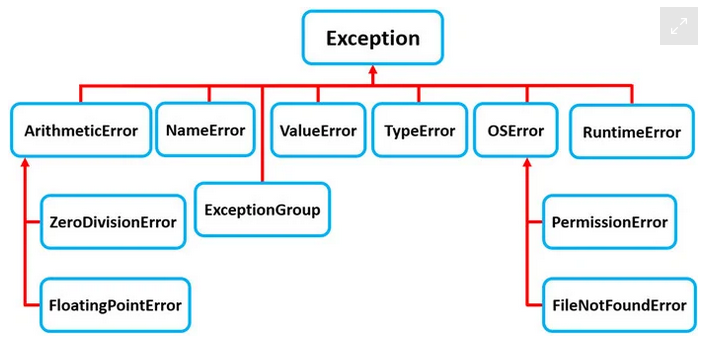
\includegraphics[width=400pt,height=260pt]{slike/class-exceptions.png}
	\caption{Klasna organizacija najvažnijih izuzetaka u programskom jeziku Pajton.}
	\label{fig: exceptions}
\end{figure}

Postoji joše jedan mehanizam koji uslovno aktivira izuzetak, a to je naredba \texttt{assert}. Ona provjerava prov da li je uslov tačan (\emph{True}). U slučaju da nije, izbacuje se poseban tip greške \texttt{AssertionError} aktivirajući navedenu poruku o grešci, gdje se potom izvršavanje narednih dijelova program zaustavlja. Primjer upotrebe naredbe \texttt{assert} je dat sljedećim k\^odom

\begin{minted}{python}
x = 5
assert x > 0, "x is not positive"
\end{minted}

Da zaključimo, rad sa izuzecima je važna praksa u pisanju robusnog koda koji je tolerantan na greške. Izuzeci nam omogućavaju elegantno rješavanje neočekivane situacije koja se javlja pri izvršavanju programa te pruža  korisniku korisne povratne informacije. 

\section{Rad sa datotekama}

Pomoću svojih ugrađenih funkcija, Pajton omogućuje jednostavan rad sa ulaznim i izlaznim datotekama. U nastavku dajemo pregled najčešće korištenih metoda.

\textit{Čitanje iz datoteke}. Koristimo funkciju \textit{open}(), koja ima dva argumenta -- naziv datoteke (ili putanja do datoteke) i način u kojem se otvara datoteka (npr. za čitanje, pisanje, dodavanje, itd.). Pogledajmo sljedeći primjer: 
\begin{minted}{python}
# Otvaranje fajla za citanje
file = open("datoteka.txt", "r")
# Citanje sadrzaja iz fajla 
sadrzaj = file.read()
# Zatvaranje fajla
file.close()
# Ispisivanje sadrzaja fajla 
print(sadrzaj)
\end{minted}

Dakle, prvo otvaramo datoteku  \texttt{datoteka.txt} samo za čitanje. Zatim čitamo sadržaj datoteke koristeći metodu \textit{read}() i čuvamo ga u varijabli \textit{sadrzaj}. Konačno, zatvaramo datoteku pomoću metode \textit{close}() i ispisujemo sadržaj datoteke. 



\textit{Pisanje u fajl}. Za pisanje u datoteku koristimo funkciju \textit{open}(), koja otvara fajl sa određenim nazivom, ali ovaj put sa načinom ``\textit{w}" (eng. \textit{write}), čime se dopušta pisanje u fajl. Pogledajmo sljedeći primjer.
\begin{minted}{python}
# Otvaranje fajla za pisanje
file = open("datoteka.txt", "w")
# Pisanje teksta u datoteku
file.write("Zdravo!")
#  Zatvaranje fajla 
file.close()
\end{minted}


\textit{Dodavanje u fajl}. Da biste dodali sadržaj u postojeći sadržaj datoteke, otvaramo fajl sa načinom ``\textit{a}" (eng. \textit{append}), a potom pomoću funkcije \textit{write}() upisujemo novi sadržaj na postojeći. 

Napomenimo da je dobra praksa zatvoriti datoteku nakon što završite rad sa njom, kako bismo izbjegli bilo kakve potencijalne probleme sa oštećenjem datoteke ili gubitkom podataka. Praksa je da se rad u fajlovima odvija pod \textit{try}-\textit{except} blokom. Klase izuzetaka koje se u tim slučajevima mogu koristiti su: \texttt{FileNotFoundError} i \texttt{OSError}. 

% Upis json, csv, ispis itd. 

\subsection{Modul Json}

Modul \texttt{json} se koristi  za enkodiranje i dekodiranje podataka sa i u JSON format (eng. \textit{Java Script Object Notation}) formatu. JSON je  široko rasprostranjen format za razmjenu podataka, ljudima jednostavan za čitanje i pisanje, a mašinama za raščlanjivanje i generisanje.

Modul \texttt{json} nudi dvije glavne metode za rad sa JSON podacima:


\begin{itemize}
	\item json.\textit{dump}() -- koristi se za enkodiranje pajton objekata u JSON format i njegovo spremanje u objekat  datoteka.
	\item json.\textit{loads}() -- koristi se za dekodiranje JSON niza u pajtonov objekat (obično heš mapa).
\end{itemize}

Pogledajmo i jedan primjer upotrebe \texttt{json} modula. 

\begin{minted}{python}
	import json
	
	# Pajton objekat
	objekat = {'ime': 'Mirko', 'godine': 30, 'grad': 'Banja Luka'}
	# Enkoduj objekat u JSON string
	json_string = json.dumps(objekat)
	# Dekodiraj JSON string nazad u pajtonov objekat (dict)
	dekodiran_objekat = json.loads(json_string)
	
	print(type(json_string))   # <class 'str'>
	print(type(dekodiran_objekat))   # <class 'dict'>
	print(dekodiran_objekat)    # {'ime': 'Mirko', 'godine': 30,
		                        # 'grad': 'Banja Luka'}
\end{minted}


Primijetite da funkcija \textit{dumps}() pretvara pajtonov objekat u string (kodiranje), dok funkcija \textit{loads}() radi obrnutu akciju, od stringa pravi pajtonov objekat (enkodiranje). 

\section{Regularni izrazi}

U ovoj sekciji izlažemo uoptšteno o regularnim izrazima. Potom, će biti riječi o Pajtonovom modulu \texttt{re} specijalno namijenjenom za rad sa regularnim izrazima. Na kraju ćemo dati nekoliko primjera upotrebe ovog modula. 

\subsection{Uopšteno o regularnim izrazima}

˘Regularni izraz ili \textit{regex} (šablon ili patern) je niz znakova koji opisuju skupove nizova znakova, na osnovu određenih žsintaksnih pravila. U prevodu to je šablon koji opisuje neki skup stringova.  Svrha regirarnih izraza je opisivanje uzorka za pretraživanje nizova znakova konciznim opisom bez nabrajanja svih elemenata (stringova) skupa. Npr. kako koncizno opisati sve binarne nizove
pomocu šablona ili kako koncizno opisati skup \{\texttt{gray}, \texttt{grey}\} (engleski i
americki engleski za istu riječ)? Regularne izraze koriste razni uređivači teksta, kao što je filter \textit{grep} u Unix-u, itd. 

Osnovni koncepti regularnih izraza su:
\begin{itemize}
	\item \textit{Alternacija} -- izražava se pomoću znaka $\mid$, te označava sve alternativne mogućnosti koje se mogu uzeti; npr. regluarni izraz $a\mid b\mid c$ označava skup riječi $\{a, b, c\}$.  
	\item \textit{Zagrada} -- označava grupisanje, tj. područje djelovanja. Npr. \texttt{gr}(a$\mid$e)\texttt{y} označava patern kojim u obuhvaćeni riječi \texttt{gray} i \texttt{grey}.
    \item \textit{Specijalni karakteri i skup karaktera}:
    \begin{itemize}
    	\item ``$.$'': sparuje bilo koji karakter samo jednom; 
    	\item $[]$: sparuje bilo koji karakter pod (uglastim) zagradama samo jednom. Npr. ako želimo da označimo skup sva malih slova, odgovarajući patern bi bio [$a-z$], dok bismo velika označili sa [$A-Z$], a jedna i druga sa [$a-zA-Z$]
    	\item $\backslash d$: sparuje bilo koju cifru samo jednom. Drugi način je koristiti patern sa zagradama: [$0-9$];
    	\item $[\^ \   ]$: sparuje bilo koji karakter tačno jednom koji pripada komplementu skupa karaktera pod
    	uglastim zagradama; 
    	\item $\backslash w$: sparuje bilo koji karakter riječi (slova, brojevi ili povlaka); 
    	\item $\backslash n$: sparuje novi red;
    	\item $\backslash s$: sparuje blanko simbol; 
    	\item $\backslash b$: sparuje granicu riječi -- položaj između znaka riječi i znaka koji nije riječ, kao što je razmak, interpunkcija oznaka ili početak/kraj reda;
    	\item $\backslash t$, $\backslash .$, $\ldots$.
    \end{itemize}
	\item  \textit{Kvantifikatori} -- navode se nakon znaka ili grupe, i oni određuju  učestalost
pojavljivanja izraza koji prethodi kvantifikatoru:
\begin{itemize}
	\item ``?'': izraz prije pojavljivanja kvantifikatora se pojavljuje 0 ili 1 puta; % -- colou?r
	\item ``*'': izraz prije pojavljivanja kvantifikatora se pojavljuje 0 ili više puta;
	\item  ``+'': izraz prije pojavljivanja kvantifikatora se pojavljuje  1 ili više puta;
	\item $\{m,n\}$: izraz prije ovog kvantifikatora se pojavljuje od $m$ do $n$ puta (uključujući i granične vrijednosti).
\end{itemize}
\end{itemize}

Reguaran izraz za registarske tablice automobila su date u formatu tri broja, potom povlaka, pa jedno (veliko) slovo, pa potom tri broja, što odgovara regularnom izrazu:
$$ \backslash d \{3\}-[A-Z]-\backslash d\{3\}$$

Regularni izraz za definisanje datum rođenja (sa vodećim nulama za jednocifreni dan i mjesec rođenja; npr. 1 se označava sa 01) izgleda ovako:
$$(\backslash d \{2\})\backslash.(\backslash d \{2\})\backslash.(\backslash d \{4\})\backslash. $$ 

\subsection{Modul Re}
Modul \texttt{re}  je ugrađeni modul koji je namijenjen za rad sa regularnim izrazima. Ovaj modul omogućuje programerima da izrade i primjenjuju regularne izraze, te da se efikasno nalaze paterni u tekstu koji se uklapaju u date izraze. 

Neke od metoda modula \texttt{re} su date u nastavku.
\begin{itemize}
	\item Metod \textit{search}(pattern, str): pretraživanje niza znakova za određen \textit{pattern} u tekstu \textit{str}.
	\item Metod \textit{match}(pattern, str): pronalaženje  uzoraka na osnovu obrasca \textit{pattern} iz niza znakova \emph{str}; vraćanje po redoslijedu pojavljivanja   uzorka se vrši primjenom funkcije \emph{group}() na objekat vraćen prethodnom funkcijom, (Vrijednost argumenta koji se prosljećuje označava redni broj uzorka koji se izdvaja.)
	
	\item Metod \textit{sub}(pattern, strChange, str): mijenja sva podudaranja obasca \textit{pattern} sa drugim nizom znakova (\textit{strChange}) u stringu {str}.
	%\item Provjera je li je niz znakova u skladu s određenim regularnim izrazom.
	\item Metod \textit{split}(pattern, str): razdvaja  niza znakova stringa \emph{str} na osnovu  obrasca \emph{pattern}, te vraća niz razdvojenih (pod)stringova.
\end{itemize}
 
 U nastavku navodimo jedan primjer primjene modula \texttt{re} i funkcije \textit{search}().
 
 \begin{minted}{python}
 	import re
 	# definiranje uzorka koji se traži
 	pattern = r'\b\w+'
 	# niz znakova za pretraživanje
 	text = 'Hello, World!'
 	# pretraživanje po obrascu
 	match = re.search(pattern, text)
 	# ispis (prvo) podudaranje
 	print(match.group()) 
\end{minted}

 Drugim riječima, odgovara bilo kojem nizu jednog ili više uzastopnih znakova riječi   kojima prethodi granica riječi (položaj između znaka riječi i znaka koji nije riječ, kao što je razmak, oznaka interpunkcije ili početak/kraj reda.
 
\section{Moduli Sys i Getopt}

\textit{Pokretanje programa preko terminala}. Pokretanje pajton skripte preko terminala se izvršava na sljedeći način:

\begin{minted}{python}
 python myscript.py arg1 arg2
\end{minted}
gdje se komanda \emph{python} (ili \textit{python3},  ako je instalirana pajtonova verzija 3.0 ili viša) postavlja preko  varijable okruženja \texttt{PYTHONPATH}. 

 Modul \texttt{sys} omogućuje pristup nekim parametrima i funkcijama specifičnim za sistem. 

Neke od često korištenih funkcija i atributa \texttt{sys} modula su:

\begin{itemize}
	\item \textit{argv}: Lista argumenata komandne linije proslijeđenih pajtonovoj skripti. Na indeksu 0 se čuva naziv same skripte, dok se na ostalim indeksima čuvaju vrijednosti proslijeđenih parametara. 
     \item \textit{path}: Vraća listu stringova koji specificiraju stazu do pojedinih modula. Inicijalizuje se iz varijable okruženja PYTHONPATH i zadate vrijednosti koja zavisi o instalaciji pajtona.
     \item \textit{exit}([arg]): Izlazak iz pajtonovog inetrpretera sa opcionim izlaznim k\^odom. Ako je dat \textit{arg}, on se koristi kao izlazni k\^od; inače je zadani izlazni kod nula.
     \item \textit{version}: Niz koji sadrži verziju pajtonovog interpretera.
     \item \textit{platform}: Niz koji identikuje platformu operativnog sustava.
\end{itemize}

U nastavku slijedi nekoliko programa koji pokazuju rad sa \texttt{sys} modulom. 

\begin{minted}{python}
import sys
if len(sys.argv) > 1:
    print("Argumenti komandne linije su:")
    for arg in sys.argv[1:]:
        print(arg)
else:
    print("Nema proslijeđenih argumenata komandne liniije.")
\end{minted}

Izvršavanjem prethodnog programa dobijamo izlaz:
\begin{minted}{python}
Argumenti komandne linije su:
arg1
arg2
\end{minted}

Modul \texttt{getopt} predstavlja parser argumenata komandne linije. Omogućuje  pisanje skripti koje mogu uzimati argumente i opcije iz komandne linije pri izvršavanju programa. Modul \textit{getopt} ima dvije bitne funkcije, \textit{getopt}() i \textit{getopt\_long}(), koje se koriste za analiziranje argumenata komandne linije. 

Funkcija \textit{getopt}() analizira kratke opcije (opcije od jednog slova) i vraća torku od dva elementa:

\begin{itemize}
	\item prvi element je lista parova (opcija, vrijednost); 
	\item drugi element je lista argumenata preostalih nakon uklanjanja opcija.
\end{itemize} 
 
Funkcija getopt\textit{\_long}(), sa druge strane, analizira duge opcije (opcije sa više slova) i vraća torku od dva elementa: 
\begin{itemize}
	\item  prvi element je lista parova (opcija, vrijednost);
	\item  drugi element je lista argumenata koja preostaje nakon uklanjanja opcija.
\end{itemize}

Kratke opcije stoje u formatu stringa slova koje odgovaraju opcijama. 
U slučaju kratkih opcija koje zahtijevaju unos vrijednosti, u nastavku stoji ``:''. 
Npr. ako imamo ``hi:o:'' koja odgovara kratkim nazivima opcija, to znači da su uz argumente -$i$ i -$o$ obavezne vrijednosti, dok argument -$h$ može da stoji samostalno. 
  
Duge opcije stoje u obliku liste naziva opcija (zapisane pomoću stringa). 
U slučaju dugih opcija koje zahtijevaju unos vrijednosti, na kraju svake opcije stoji ``=''.  U nastavku slijedi primjer korišćenja modula \texttt{getopt}.

\begin{minted}{python}
import getopt
import sys

def main(argv):
    inputfile = outputfile = ''
    try:
        opts, args = getopt.getopt(argv,"hi:o:",["ifile=","ofile="])
    except getopt.GetoptError:
        print('test.py -i <inputfile> -o <outputfile>')
        sys.exit(2)
    for opt, arg in opts:
        if opt == '-h':
                print('test.py -i <inputfile> -o <outputfile>')
                sys.exit()
        elif opt in ("-i", "--ifile"):
                inputfile = arg
        elif opt in ("-o", "--ofile"):
                outputfile = arg

print('Ulazni fajl je:' , inputfile)
print('Izlazni fajl je: ', outputfile)

if __name__ == "__main__":
    main(sys.argv[1:])
\end{minted}
U prethodnom primjeru, skripta uzima dva argumenta, -$i$ (ili duže - -\emph{ifile}) za ulazni fajl, te -$o$ (ili duže - -\emph{ofile}) 
za izlazni fajl. U slučaju da korisnik ne proslijedi (obavezne) argumente, skripta će ispisati poruku o greški -- aktiviraće se izuzetak \texttt{GetoptError} koji pripada modulu \texttt{getopt}. 

 Da bi pokrenuli skriptu (naziva test.py), na komandnoj liniji unosimo sljedeći kod:
 \begin{minted}{python}
python3 test.py -i ulaz.txt -o izlaz.txt
 \end{minted}
 Nakon pokretanja skripte, prikazaće se sljedeće:
\begin{minted}{python}
Ulazni fajl je ulaz.txt
Izlazni fajl je izlaz.txt
 \end{minted}

\section{Modul Numpy}

Ovaj modul je specijalizovan za rad sa nizovima i nizovnim strukturama kao što su
matrice, 3D matrice, proizvoljne matrice,  velikih dimenzija. Riječ \texttt{numpy} predstavlja skraćenicu  engleske fraze \emph{numerical python}.  Kreirana je 2005. od strane Travisa Oliphanta, a napisana je u jezicima C/C++. Jedan numpy  objekat predstavlja neprekidan (statičan) dio u memoriji, a za razliku od liste, ovaj objekat je homogene strukture, vidjeti Sliku 	\ref{fig:numpy_array}. Zbog svega toga, pogodan je   za rad  sa velikim tipovima podataka, i brži je što je tiče osnovnih operacija za red velicine (oko 50 puta) od tradicionalne liste.

\begin{figure}%https://stackoverflow.com/questions/57262885/how-is-the-memory-allocated-for-numpy-arrays-in-python
	\centering
	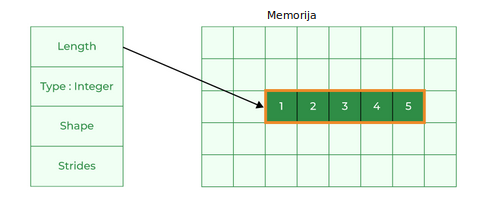
\includegraphics[width=320pt,height=170pt]{slike/numpy-array-memory.png} %numpy_array.png}

	\caption{Struktura podataka numpy niza (sa tipom podataka $int$).\protect \footnotemark}	 \label{fig:numpy_array}
 
\end{figure} 
\footnotetext{https://www.geeksforgeeks.org/python-lists-vs-numpy-arrays/}

\textit{Inicijalizacija objekta}. 
\begin{minted}{python}
import numpy as np
ar = np.array([2, 4, 1, 10], dtype="int32") # niz
matrica = np.array([[2, 5 ], [1, 7] ], dytpe="int32") # matrica (2D-niz)
matrica3D = np.array( [[[2, 5 ], [1, 7] ], [[2, 3], [5, 5]]], \ 
dytpe="int32") # 3D matrica
\end{minted}
 
Što se tiče eksplicitno definisanog tipa elemenata objekta numpy (argument \emph{dtype}) mogući su sljedeći tipovi:  $i$: integer (i4, i2, itd.),  $b$: boolean, $u$: unsigned integer, $f$: float,  $M$: datetime, $O$: object, $S$: string. 

\textit{Osnovne metode}.
\begin{itemize}
	\item  Vraćanje elementa na određenoj poziciji (indeksu): 
	\begin{itemize}
		\item 1D niz:  [indeks]
		\item 2D niz:  [indeks1, indeks2]
		\item 3D niz: [indeks1, indeks2, indeks3]
	\end{itemize}
    \item \textit{shape}(): vraćanje dimenzije niza;  
    \item Izrezivanje (\textit{slicing}):  [start:end:step]: slično kao i kod listi; 
    \item Kopiranje niza: funkcija \textit{copy}() koja se primjenjuje na objekat koji se kopira (tačka notacija);
    \item \textit{reshape}(): promjena dimenzije niza, potrebna je kompatibilnost broja
    elemenata početnog niza sa izmijenjenom dimenzijom; 
    \item \textit{np.concatenate}( ($arr1, arr2$), $axis=$.): spajanje dva numpy objekta   
    po $x$ ili $y$ osi (argument axis ili 0 ili 1) 
    \item  \textit{np.array\_split}($arr, n, axis$): dijeljenje niza \textit{arr} na više manjih nizova, gdje je $n$ broj nizova na koje dijelimo niz, dok je  \textit{axis} osa po kojoj želimo da vršimo dijeljenje;
    \item  \textit{where}(uslov): vraća niz indeksa onih elemenata niza koji se uklapaju u \textit{uslov}; npr. uslov može biti: $arr$== 4 ili $arr$ \% 2 == 0;
    \item \textit{np.sort}(\emph{arr}): sortiranje niza \emph{arr};
    \item Filtriranje elemenata u nizu se može izvesti na sljedeći način
    \begin{minted}{python}
arr = np.array([41, 42, 43, 44])
filter_arr = arr > 42
newarr = arr[filter_arr]
    \end{minted}
    \item \textit{numy.zeros}(dim), \textit{numpy.ones}(dim): kreiranje matrice dimenzije dim sa svim nulama, odnosno jedinicama.
\end{itemize}

 \textit{Memorijska organizacija}. Slika~\ref{fig:numpy_array} daje pojednostavljeni prikaz memorijske organizacije numpy objekta u jeziku Pajton.  Ovaj objekat pripada klasi \texttt{ndarray}, koja ima nekoliko bitnih atributa: 
 \begin{itemize}
 	\item \textit{dtype}: definiše tip podataka elemenata koji se smještaju u strukturi.
 	\item \textit{dim\_count}: definiše dimenzionalnost objekta (2D, 3D, isl.).  
 	\item \textit{dimensions}: definiše dimenzije po svakoj od koordinata.  
 	\item \textit{strides}: torka koja definiše broj bajtova koje treba pomaknuti u memoriji da bi se pristupilo sljedećem elementu u nizu duž određene dimenzije. Npr. za 2D niz, \textit{stride} torka je definisana sa (bajt\_za\_pomicanje\_u\_smjeru\_reda, bajt\_za\_pomicanje\_u\_smjeru\_kolone). 
 	\item \textit{data}: pokazivač na sadržaj niza. 
 \end{itemize} 
 

\section{Modul Ctypes}

Modul \textit{ctypes} pruža način za pozivanje funkcija i korištenje tipova podataka u dijeljenim  bibliotekama ili bibliotekama dinamičkog povezivanja (DLL) napisanim u jeziku \textit{C} ili drugim jezicima nižeg nivoa unutar pajtonovog koda. Osnovni  koraci za korištenje \textit{ctypes} modula za uključivanje \textit{C} programa u pajtonov k\^od su dati u nastavku.

\begin{enumerate}
	\item Prvo  napisati \textit{C} program koji želimo ugraditi u pajtonov   k\^od. Ovaj program može da sadrži jednu ili više funkcija koje želimo pozvati unutar k\^oda pisanog u Pajtonu.
	\item Prevesti (kompajlirati) \textit{C} program u dijeljenu biblioteku.    Na Linuks ili macOS  sistemima u tu svrhu koristimo \textit{gcc} kompajler. Na sistemu Windows možete koristiti Visual Studio ili MinGW za kompajliranje programa u DLL fajl.
	\item Učitati dijeljenu biblioteku u pajtonov k\^od. Ovaj proces vršimo uz  pomoć modula \texttt{ctypes}. Učitavamo .dll fajl pozivanjem \textit{cdll.LoadLibrary(path)} gdje je \textit{path} proslijeđena staza do dijeljene (dll) biblioteke.
	\item Definišimo tipove argumenata i ono što vraćaju funkcije napisane u \textit{C} programu. Prije nego što   pozovemo \textit{C} funkciju iz pajton programa pomoću modula \texttt{ctypes}, trebaju se navesti tipovi argumenata i tipovi koje funkcije vraćaju. To možemo učiniti postavljanjem \textit{argtypes} i \textit{restype} atributa funkcijskog objekta.
	\item Pozivanje \textit{C} funkcije u pajtonovom programu: Na kraju, pozivamo \textit{C} funkciju iz pajtona pomoću funkcijskog objekta koji je kreiran u koraku 4. Vrijednosti argumenata proslijeđujemo kao pajtonove objekte, a modul \texttt{ctypes} će ih automatski pretvoriti u odgovarajuće \textit{C} tipove podataka. 
\end{enumerate}

U nastavku navodimo čitav proces   poziva \textit{C} programa izvršavanjem pajtonovog koda.


\begin{minted}{C}
	// dodaj.c
	int saberi(int a, int b) {
		return a + b;
	}
\end{minted}

Kompajlirajmo \textit{C} k\^od pomoću \textit{gcc} kompajlera:
\begin{minted}{C}
	  gcc -shared -o lib_dodaj.so dodaj.c
\end{minted}
Dalje, učitavamo kreirani dijeljeni fajl u pajtonov program pomoću  \texttt{ctypes} modula:
\begin{minted}{python}
	import ctypes
	lib_dodaj = ctypes.cdll.LoadLibrary('./lib_dodaj.so')
\end{minted}
Potom, eksplicitno definišemo tipove argumenata i tip koji vraća odabrana \textit{C} funkcija:
\begin{minted}{python}
	saberi_func = lib_dodaj.saberi
	saberi_func.argtypes = [ctypes.c_int, ctypes.c_int]
	saberi_func.restype = ctypes.c_int
\end{minted}
Konačno, pozovemo odabranu \textit{C} funkciju uz pomoć k\^oda:
\begin{minted}{python}
	result = saberi_func(2, 3)
	print(result)   # Output: 5
\end{minted}

 
\section{Pisanje prilagodjenih modula}

Pretpostavimo da želimo kreirati modul koji služi za različite matematičke operacije, kao što su sabiranje, oduzimanje, množenje i dijeljenje. Kako smo pomenuli, modul je skup objekata koji se  čuva u datoteku ekstenzije .\textit{py}. Pretpostavimo da želimo kreirati modul pod nazivom \textit{mathOps}. Dakle, kreirajmo  datoteku pod nazivom ``\textit{mathOps}.py" u kojem definišemo funkcije ovog prilagodjenog modula. Evo primjera kako bi ta datoteka mogla izgledati:

\begin{minted}{python}
def add(x, y):
    return x + y

def subtract(x, y):
    return x - y

def multiply(x, y):
    return x * y

def divide(x, y):
    if y == 0:
        raise ValueError("Ne možemo dijeliti sa 0")
    return x / y
\end{minted}
Ovaj  primjer definiše četiri različite funkcije, od kojih svaka izvodi različite matematičke operacije. Funkcija \textit{add} uzima vrijednost dva argumenta, $x$ i $y$, i vraća njihov zbir. Funkcija \textit{subtract}   vraća razliku dva broja koji se prenose kao argumenti funkcije. Funkcija \textit{multiply} vraća proizvod dva broja. Konačno, funkcija \textit{divide} uzima dva argumenta, i vraća rezultat njihovog dijeljenja, ali takođe  javlja  grešku ako je nazivnik (vrijednost argumenta $y$) nula.

Korištenje ovog prilagodjenog modula u drugoj pajtonovoj datoteci se vrši importovanjem modula \textit{mathOps} na sljedeći način:

\begin{minted}{python}
import mathOps

result = mathOps.add(3, 4)
print(result)   # Output: 7

result = mathOps.divide(10, 2)
print(result)   # Output: 5.0

result = mathOps.divide(10, 0)
# Output: ValueError: Ne možemo dijeliti sa 0
\end{minted}

U ovom primjeru uvozimo modul ``\textit{mathOps}" i koristimo njegove funkcije za izvođenje matematičkih operacija. Pozivamo funkciju  \textit{add}  koja vraća zbir brojeva 3 i 4, a to je 7. Zatim pozivamo funkciju  \textit{divide}  za dijeljenje 10 sa 2, koja vraća 5.0. Na kraju, ponovno pozivamo funkciju  \textit{divide}  da bismo podijelili 10 sa 0, što uzrokuje \texttt{ValueError} jer dijeljenje sa nulom nije dopušteno.


\section{Postavljanje korisnički kreiranih modula  na PyPI repozitorij}

PyPI (\textit{Python Package Index}) je centralni repozitorij paketa   koji su pisani u programskom jeziku Pajton. PyPI omogućuje programerima lako distribuiranje korisnički napisanih modula,  omogućavajući da dati paket bude korišten široj zajednici korisnika.
 
Nekoliko   koraka   treba izvršiti ukoliko želimo postaviti   korisnički kreirani modul na PyPI repozitorij. Na zvaničnoj PyPI veb stranici, na linku  \url{https://pypi.org/account/register/},  potrebno je kreirati račun. Nakon što se prijavimo, potrebno je  generisati token za prijavu na PyPI. Token je sigurnosni ključ koji omogućuje da se prijavimo i objavimo/podignemo  paket (modul). 
 
 
 Na lokalnom računaru instalirajmo module  \texttt{setuptools} i \texttt{wheel}, u slučaju da nisu instalirani. To se možete učiniti pomoću \textit{pip} naredbe:
 \begin{minted}{python}
      pip install setuptools wheel
 \end{minted}

Modul \texttt{setuptools} omogućuje da upravljamo i distribuiramo naš modul, a modul \texttt{wheel}   omogućuje generisanje datoteka sa ekstenzijom .\textit{whl} koje se mogu lako instalirati.

Potom,  u korjenom direktorijumu našeg modula  kreiramo fajl \textit{setup.py}. Fajl \textit{setup.py}  definiše metapodatke o našem modulu kao što su naziv, verzija, autor, opis i druge metapodatke koji će biti prikazani na PyPI stranici   modula. Primjer takvog fajla je dat u nastavku.

\begin{minted}{python}
   from setuptools import setup
   
   setup(
     name='modul1',
     version='0.0.1',
     author='Mirko Mirkovic',
     description='modul1',
     packages=['modul1'],
     install_requires=[
       'numpy',
       'pandas'
     ]
   )
\end{minted}
Ovaj \textit{ setup.py}   definiše paket modul1 sa verzijom 0.0.1, datim autorom  i opisom, a zavisi od modula \textit{numpy} i \textit{pandas}.

Naredni korak je kreiranje distribucijske datoteke (source distribution i wheel distribution) pomoću \texttt{setuptools}, izvršavajući naredbu:
\begin{minted}{python}
        python setup.py sdist bdist_wheel
\end{minted}
 
Dalje instaliramo \texttt{twine} paket, koji će pomoći da postavimo naš distribucijski modul na PyPI repozitorijum. Instaliramo ga pomoću   naredbe:
\begin{minted}{python}
	pip install twine
\end{minted}
Potom postavimo korisnički   modul na PyPI pomoću twine naredbe:
\begin{minted}{python}
	twine upload dist/*
\end{minted}
Izvršavanje prethodne naredba će tražiti da se unese PyPI korisničko ime i lozinka, a zatim će prenijeti      paket na PyPI (direktorijum dist).

Nakon  objave  modula na PyPI, možemo ga instalirati pomoću   naredbe:
\begin{minted}{python}
	pip install modul1
\end{minted}


\section*{Zadaci}
%regularni izrazi:
\begin{enumerate}
    %%https://adriann.github.io/programming_problems.html
    
    \item Implementirajte igru pogađanja u kojoj korisnik treba da pogodi skriveni broj. Nakon pogađanja, program izvještava korisnika da li je njegov broj velik ili mali (ili je pogođen). Na kraju ispisati broj  pokušaja iz kojeg je korisnik pogodio skriveni broj. Računa se jedan pokušaj ukoliko se unese isti broj više puta uzastopno.
    
    
	\item Napisati program koji računa sljedeću sumu  
	
	$$ 4 \cdot \sum_{k=1}^{10^6}(-1)^{k-1} \frac{1}{2k-1}= 4 \cdot (1-1/3 + 1/5-1/7+1/9-1/11 \ldots).$$
	
	\item Napisati funkciju koja kombinira dvije liste naizmjenično uzimajući naizmjenično elemente jedne pa druge liste, Npr. za $[a,b,c], [5, 6, 7]$ generišemo listu $[a,5,b,6,c,7]$.
	
	\item Napisati funkciju koja pomijera listu za $k$ elemenata. Npr. lista  $[1,2,3,4,5,6]$ rotirano za $k=2$ je data sa $[3,4,5,6,1,2]$. Riješiti zadatak bez kreiranja kopije liste. 
	
	\item Napisati funkciju koja uzima broj i vraća listu njegovih brojeva. Npr. za broj $2342$ treba vratiti listu $[2,3,4,2]$.
	
	\item Napisati funkciju koja uzima listu brojeva,   bazu $b_1$ u kojoj se brojevi liste interpretiraju, te ciljnu bazu $b_2$.  Kao rezultat vratiti listu brojeva konvertujući svaki od brojeva početne liste u bazu $b_2$. Npr. za listu $[21,10,01]$ u bazi $b_1 = 3$ pretvaramo u listu brojeva po bazi $b_2=10$, dobijajući $[7,3, 1]$.
	
	\item Napišite funkciju koja množi dvije matrice. Vratiti grešku (koristiti izuzetke) ukoliko su dimenzije matrica nekompatibilne.  
	 
	\item Napisati regularni izraz koji prepoznaje registarske tablice. Testirati primjenu uz pomoć modula \texttt{re}.
	
	\item Napisati regularni izraz koji prepoznaje imejlove. Testirati primjenu uz pomoć modula \texttt{re}.
	
	\item Napisati regularni izraz koji prepoznaje realne brojeve (u decimalnom ili eksponencijalnom zapisu). Testirati primjenu uz pomoć modula \texttt{re}.
	
	
	\item Kreirati datoteku \textit{apsolventi}.txt i popuniti je podacima gdje je u svakom redu data
	informacija o studentu apsolventu u formi: 
	 $$<Ime\_prezime>, <datum\_upisa\_na\_fakultet>, <godine\_starosti>$$ 
	
	Datum se zadaje u formi $<$broj$>$.$<$broj$>$.$<$broj$>$. Napisati skriptu koja se pokreće sa terminala čiji su argumenti komandne linije:
	\begin{itemize}
		\item  	\textit{i}: koja zadaje ulazni datoteku (sve zajedno sa putanjom) koja treba da bude učitana u
	program;
	     \item \textit{o}: koja zadaje izlaznu datoteku (sve zajedno sa putanjom) u kojoj se čuvaju rezultati	izvršavanja programa;
	     \item  \textit{z}: koji zadaje zadatak koji treba da bude izvršen i obuhvata sljedeći opseg vrijednosti: 
	     \begin{itemize}
	     	\item  1: U izlaznoj datoteci treba da se ispišu svi apsolventi stariji od 25 godina.
             \item 2: U izlaznoj datoteci treba da se ispišu svi apsolventi koji su upisali fakultet u periodu od 01.01.2014. do 01.01.2015. godine.
	         \item 3: U izlaznoj datoteci treba da se ispiše sortiran niz (koristiti merge sort) studenata po godini života.
	         \item 4: U izlaznoj datoteci treba da se ispiše za svakog studenta koliko godina studira/je studirao.
	        \item Za ostale inpute javiti poruku o neispravnoj opciji (unosu). Koristiti izuzetke.
	         \end{itemize}
       \end{itemize}
	\textit{Napomena}. Studenta učitati uz pomoć regularnih izraza. Dakle, prazni karakter je
	invarijantna vrijednost što se postiže konstrukcijom odgovarajućeg regularnog izraza pri čitanju redova iz datoteke.
	
   \item Kreirati datoteku \emph{pretplatnik.txt} i popuniti je podacima gdje je u svakom redu
   data informacija o studentu u formi
   
   $$<Ime\_prezime>, <datum\_ugovora>, <cijena\_usluge>$$
   
   Datum se zadaje u formi $<$broj$>$.$<$broj$>$.$<$broj$>$, a cijena je decimalni broj. Napisati 
   skriptu koja se pokreće sa terminala sa sljedećim argumentima komandne linije:
   \begin{itemize}
   	\item \textit{i}: koja zadaje ulaznu datoteku (sve zajedno sa putanjom) koja treba da bude učitana
   u program;
   \item \textit{o}: koja zadaje izlaznu datoteku (sve zajedno sa putanjom) koja treba da sačuva
   rezultate izvršavanja programa;
    \item \textit{z}: koji zadaje zadatak koji treba da bude izvršen i obuhvata sljedeće vrijednosti:
    \begin{itemize}
    	\item  1: U izlaznoj datoteci treba da se ispišu svi korisnici koji koriste usluge čija je  cijena veća od 15.4 KM. Eliminisati duplikate. 
        \item 2: U izlaznoj datoteci treba da se ispišu svi pretplatnici koji su potpisali ugovor u periodu od 01.01.2022. do 15.01.2023. godine.
        \item  3: U izlaznoj datoteci treba da se ispiše zbir svih cijena za usluge koje koristi svaki od pretplatnika. 
        \item 4: U izlaznoj datoteci treba da se ispišu sortirane cijene od najmanje do  najveće.
        \item Za ostale inpute javiti poruku o neispravnoj opciji  (unosu) koristeći izuzetke.
         \end{itemize}
   \end{itemize}
   \textit{Napomena}. Pretplatnika učitati uz pomoć regularnih izraza. Npr., smatra se da je unos Marko
   Markovic, $20.2.2022, 8,4$ isti kao Marko Markovic, $20.\ \ 2.2022, 8,\ \ 4$, itd. Dakle, prazni
   karakter je invarijantna vrijednost što se postiže konstrukcijom odgovarajućeg regularnog izraza
   pri čitanju redova u datoteci.
\end{enumerate}